% ============================================================
% Informe de Propuesta de Doctorado — BIP 2026
% Cross-Modal Representation Disagreement as a Lightweight
% Uncertainty Signal for Glaucoma Detection in Medical
% Vision-Language Models
%
% Autor: Miguel Guillermo Abreu Cárdenas
% Tutor: Saúl Calderón Ramírez
% Compilar con: pdflatex (dos pasadas por las referencias cruzadas)
% Las figuras se resuelven relativas a este archivo: assets/...
% ============================================================
\documentclass[12pt,a4paper]{article}

% ------------------------------------------------------------
% PAQUETES
% ------------------------------------------------------------
\usepackage[utf8]{inputenc}
\usepackage[T1]{fontenc}
\usepackage[spanish,es-nodecimaldot]{babel}
\usepackage{amsmath,amssymb,amsthm}
\usepackage{graphicx}
\usepackage{booktabs}
\usepackage{multirow}
\usepackage{array}
\usepackage{tabularx}
\usepackage{float}
\usepackage{enumitem}
\usepackage{xcolor}
\usepackage{fancyhdr}
\usepackage{geometry}
\usepackage{setspace}
\usepackage{titlesec}
\usepackage[colorlinks=true,linkcolor=blue!50!black,citecolor=blue!50!black,urlcolor=blue!50!black]{hyperref}

% ------------------------------------------------------------
% CONFIGURACIÓN DE PÁGINA Y ESTILO
% ------------------------------------------------------------
\geometry{left=2.5cm,right=2.5cm,top=2.5cm,bottom=2.5cm}
\setstretch{1.15}
\setlength{\parskip}{0.35em}

\pagestyle{fancy}
\fancyhf{}
\fancyhead[L]{\small Informe de Propuesta de Doctorado --- BIP 2026}
\fancyhead[R]{\small\nouppercase{\leftmark}}
\fancyfoot[C]{\thepage}
\renewcommand{\headrulewidth}{0.4pt}

\titleformat{\section}{\Large\bfseries}{\thesection.}{0.5em}{}
\titleformat{\subsection}{\large\bfseries}{\thesubsection.}{0.5em}{}
\titleformat{\subsubsection}{\normalsize\bfseries}{\thesubsubsection.}{0.5em}{}

% Comandos de conveniencia (nombres científicos fijados del proyecto)
\newcommand{\pvis}{p_{\mathrm{vis}}}
\newcommand{\ptext}{p_{\mathrm{text}}}
\newcommand{\ux}{u(x)}
\newcommand{\KL}{D_{\mathrm{KL}}}

% ============================================================
\begin{document}

% ------------------------------------------------------------
% PORTADA
% ------------------------------------------------------------
\begin{titlepage}
    \centering
    \vspace*{1.5cm}
    {\large Doctorado en Inteligencia Artificial aplicada a Oftalmología\par}
    \vspace{1.2cm}
    {\LARGE\bfseries Informe de Propuesta de Doctorado\par}
    \vspace{0.8cm}
    {\large\itshape Cross-Modal Representation Disagreement as a Lightweight
    Uncertainty Signal for Glaucoma Detection in Medical Vision-Language Models\par}
    \vspace{0.6cm}
    {\large (Desacuerdo de representación cross-modal como señal ligera de
    incertidumbre para la detección de glaucoma en modelos médicos
    visión-lenguaje)\par}
    \vfill
    \begin{tabular}{rl}
        \textbf{Autor:} & Miguel Guillermo Abreu Cárdenas \\
        \textbf{Tutor:} & Saúl Calderón Ramírez \\
        \textbf{Fecha:} & Agosto de 2026 \\
        \textbf{Estado:} & Fase 1 del experimento completada y verificada \\
    \end{tabular}
    \vspace{1.5cm}
\end{titlepage}

% ------------------------------------------------------------
% RESUMEN
% ------------------------------------------------------------
\begin{abstract}
\noindent
Los Vision-Language Models (VLMs) médicos como MedGemma-4B comienzan a
usarse para pre-clasificar imágenes diagnósticas, pero carecen de todo
mecanismo nativo para \emph{saber cuándo no saben}: en nuestros
experimentos, MedGemma declara una confianza verbalizada de 95\% en el
91.5\% de las imágenes mientras acierta solo el 79.8\% de los casos. Este
informe presenta la propuesta doctoral y su primera fase experimental
completada: una señal de cuantificación de incertidumbre (UQ) basada en el
\emph{desacuerdo de representación cross-modal} --- la divergencia de
Kullback-Leibler (KL) entre los hidden states de los tokens de imagen y el
estado que condiciona el token de respuesta, en la última capa del decoder
del propio VLM --- extraída del \textbf{mismo forward pass} que produce la
respuesta, sin entrenar ni calibrar nada (\emph{training-free},
\emph{single-pass}, costo computacional 1$\times$).

Sobre el dataset MM-ODIR-129 (129 fotografías de fondo de ojo, 60 Normal /
69 glaucoma, re-anotadas por oftalmólogos), la señal
$\ux = \KL(\ptext \Vert \pvis)$ detecta los errores del modelo con
AUROC $= 0.661$, IC 95\% $[0.522, 0.772]$ (bootstrap BCa), $p = 0.006$
(Mann-Whitney), verificando la hipótesis principal H1. Una fusión original
y libre de parámetros, $\mathrm{rank}(\mathrm{KL}) +
\mathrm{rank}(1-\mathrm{MSP})$, mejora la detección a AUROC $= 0.698$ y
reduce el riesgo de selective prediction (Excess-AURC $= 0.407$ frente a
$0.670$ de la KL sola), habilitando un esquema clínico de triage en tres
zonas en el que el 30.2\% menos incierto de la cohorte no contiene ningún
error del modelo. La señal domina en el frente de Pareto a los baselines
multi-pass de mayor costo (confianza verbalizada 2$\times$: AUROC $0.519$;
self-consistency 10$\times$: AUROC $0.655$). La hipótesis exploratoria H4
(correlación con la severidad del glaucoma) fue rechazada
($\rho = +0.001$, $p = 0.99$): la señal detecta errores del modelo, no
gravedad de la enfermedad. El pipeline completo fue verificado con código
independiente (19/19 checks) y re-ejecución cross-GPU (logits bitwise
idénticos). El documento detalla los objetivos del doctorado, la revisión
de la literatura, la metodología, la propuesta por fases y una sección
extensa de resultados con su interpretación.

\medskip
\noindent\textbf{Palabras clave:} cuantificación de incertidumbre (UQ),
Vision-Language Models, MedGemma, divergencia KL cross-modal, hidden
states, selective prediction, glaucoma, retinografía, triage clínico.
\end{abstract}

\newpage
\tableofcontents
\newpage

% ============================================================
\section{Resumen de la propuesta}
% ============================================================

\subsection{Problema y motivación}

El glaucoma es una neuropatía óptica progresiva y una de las principales
causas de ceguera irreversible en el mundo. Es asintomático hasta etapas
avanzadas, de modo que el \emph{screening} por fotografía de fondo de ojo
es la intervención de mayor impacto: detectarlo temprano frena la pérdida
visual. Los VLMs médicos recientes ---MedGemma de Google Research entre
ellos--- alcanzan desempeños competitivos en benchmarks de imagen médica,
lo que abre la puerta a un escenario de \emph{triage automatizado}: un
modelo que pre-clasifica imágenes de screening y deriva al oftalmólogo
solo los casos dudosos.

Ese escenario choca con un hecho empírico incómodo: \textbf{el modelo es
un mal juez de sí mismo}. En nuestros experimentos sobre 129 retinografías,
MedGemma-4B acierta el 79.8\% de las clasificaciones glaucoma/normal, pero
la mediana de su probabilidad de respuesta entre los casos que afirma es
$\approx 0.9999$ (nunca ``duda'' en su output), y cuando se le pregunta
directamente su confianza, solo declara dos valores ---95 y 90 sobre
100--- con una accuracy real de 80.5\% cuando dice 95. Un sistema de triage
que confiara en la confianza declarada o en los logits de salida derivaría
casos esencialmente al azar.

\subsection{Idea central}

La propuesta explota una propiedad estructural de los VLMs: durante el
forward pass, los hidden states de las posiciones de imagen y los de las
posiciones de texto \emph{evolucionan dentro del mismo espacio vectorial}
del decoder, capa a capa, influenciándose mutuamente por la atención. En la
última capa, el estado del token que está a punto de generar la respuesta
(``yes''/``no'') y los estados de los 256 tokens de imagen son, formalmente,
\textbf{dos vistas del mismo caso clínico escritas en el mismo idioma
vectorial} --- y por tanto comparables directamente con una divergencia
entre distribuciones.

La intuición clínica es simple: cuando el modelo procesa un caso que
domina, sus dos ``voces internas'' ---la visual y la textual--- convergen;
cuando el caso es ambiguo o el modelo se equivoca, esa convergencia se
rompe y el texto afirma con seguridad algo que la imagen no respalda. Si
esa ruptura se puede medir, hay una alarma. La medimos con la divergencia
KL entre ambas representaciones, extraída del \textbf{mismo forward pass}
que produce la respuesta: sin entrenamiento, sin calibración, sin muestreos
múltiples, a costo computacional 1$\times$.

\subsection{Contribuciones verificadas como originales}

Un análisis de novedad (verificado por especialista externo mediante
búsqueda exhaustiva) estableció que la combinación
\emph{MedGemma-4B + divergencia KL cross-modal en un solo forward pass +
UQ para glaucoma} no existe previamente en la literatura. Las dos
contribuciones originales de esta fase doctoral son:

\begin{enumerate}[leftmargin=1.6em]
    \item \textbf{Señal KL cross-modal intra-modelo:} primer método de UQ
    que es simultáneamente \emph{single-pass}, \emph{training-free} y
    \emph{cross-modal}. Nadie antes extrajo la divergencia KL entre los
    hidden states de los tokens visuales y el estado textual del decoder
    de un VLM como señal de incertidumbre. Resultado: AUROC $0.661$
    $[0.522, 0.772]$, $p = 0.006$, con dominancia Pareto sobre todos los
    baselines multi-pass (2$\times$ y 10$\times$).
    \item \textbf{Fusión \emph{parameter-free}
    $\mathrm{rank}(\mathrm{KL}) + \mathrm{rank}(1-\mathrm{MSP})$:} primera
    combinación por agregación de rangos de una señal del espacio de
    representaciones internas (KL cross-modal) con una señal del espacio
    de salida (MSP) para UQ en VLMs. La técnica genérica de agregación por
    ranks proviene de information retrieval (Cormack et al., 2009), pero
    su instanciación para fusionar señales de UQ heterogéneas en VLMs es
    nueva. Resultado: AUROC $0.698$, Excess-AURC $0.407$ (un 39\% más
    cerca del oracle que la KL sola), y una ``zona verde'' del 30.2\% de
    la cohorte sin errores.
\end{enumerate}

\subsection{Alcance de este informe}

Este documento presenta: (i) los objetivos del proyecto doctoral y su
articulación por fases; (ii) la revisión de la literatura que delimita el
nicho de la contribución; (iii) la descripción completa de la metodología
(definición formal de la señal, dataset, protocolo, métricas); (iv) la
propuesta detallada ---qué se quiere hacer y cómo--- incluyendo el roadmap
doctoral; y (v) una sección extensa de resultados obtenidos en la Fase 1,
con su interpretación, su forma de obtención y sus limitaciones. La Fase 1
está \textbf{completada y verificada}; las fases siguientes constituyen el
trabajo por realizar hasta la defensa.

% ============================================================
\section{Objetivos}
% ============================================================

\subsection{Objetivo general}

Desarrollar y validar métodos de cuantificación de incertidumbre (UQ) y
explicabilidad (XAI) que operen sobre las capas y módulos internos de
modelos médicos visión-lenguaje, de modo que un sistema de screening
oftalmológico automatizado pueda \emph{saber cuándo no sabe} y derivar
esos casos al especialista, comenzando por la detección de glaucoma en
retinografía como caso de estudio principal.

\subsection{Objetivos específicos}

\begin{enumerate}[leftmargin=1.6em]
    \item \textbf{[Fase 1 --- completada]} Demostrar que el desacuerdo
    entre la representación visual y la representación textual interna de
    un VLM médico (\emph{cross-modal representation disagreement}), medido
    por divergencia KL en un solo forward pass y sin entrenamiento, es una
    señal de alarma de error estadísticamente significativa (meta de
    diseño: AUROC $\geq 0.65$ con IC bootstrap 95\% reportado
    honestamente).
    \item \textbf{[Fase 1 --- completada]} Evaluar esa señal contra
    baselines de igual costo (entropy, $1-\mathrm{MSP}$, energy) y de
    mayor costo (confianza verbalizada 2$\times$, self-consistency
    10$\times$), y cuantificar su utilidad clínica en el marco de
    \emph{selective prediction} (curvas accuracy-coverage, AURC, triage
    por percentiles).
    \item \textbf{[Fase 1 --- completada]} Diseñar una fusión libre de
    parámetros que combine la señal interna cross-modal con la confianza
    de salida, y verificar su complementariedad empírica.
    \item \textbf{[Fase 2]} Escalar la validación a datasets grandes
    (Harvard-FairVLMed, 10\,000 imágenes; RIM-ONE, REFUGE, ORIGA) y a
    otros VLMs médicos (LLaVA-Med, CogVLM) para determinar si la señal es
    propiedad del mecanismo o del modelo.
    \item \textbf{[Fase 3]} Generalizar a otras tareas médicas de
    screening y profundizar en la estructura interna de la señal:
    \emph{signature maps}, barrido fino de capas (27--34), selección de
    capas óptimas y early-exit como extensión de eficiencia.
    \item \textbf{[Fase 4]} Integrar el esquema de triage en tres zonas en
    un flujo clínico oftalmológico real (estudio prospectivo) y
    complementarlo con una capa de explicación al oftalmólogo (Grad-CAM /
    Integrated Gradients sobre los casos derivados), articulando UQ + XAI
    como contribución doctoral completa.
\end{enumerate}

% ============================================================
\section{Revisión de la literatura}
% ============================================================

\subsection{Vision-Language Models y MedGemma}

Un VLM moderno combina tres piezas: un \emph{vision encoder} (un Vision
Transformer entrenado con contraste imagen-texto, al estilo CLIP/SigLIP),
un \emph{proyector} que mapea las representaciones visuales al espacio de
embeddings del modelo de lenguaje, y un \emph{decoder} autorregresivo que
trata los tokens de imagen proyectados como parte de su secuencia de
entrada. Familias representativas: LLaVA, CogVLM, Qwen-VL y los Gemma 3
multimodales. En el dominio médico destacan LLaVA-Med (Li et al., 2023),
RadFM, Med-Flamingo y MedGemma (Sellergren et al., 2025).

MedGemma-4B (\texttt{google/medgemma-4b-it}) combina: (i)
\textbf{MedSigLIP}, un vision encoder SigLIP ($\sim$400M parámetros)
adaptado a imagen médica que produce 256 tokens de imagen a partir de
entradas de $896\times896$ px; (ii) un \textbf{proyector} que lleva cada
token visual de 1152 dimensiones a las 2560 del espacio del decoder; y
(iii) el \textbf{decoder Gemma 3}: 34 capas de transformer decoder-only,
dimensión oculta 2560, atención causal. Sus reportes técnicos documentan
mejoras sustanciales en benchmarks médicos, pero \textbf{no incorporan
ningún mecanismo nativo de UQ} --- y mucho menos uno basado en comparar
representaciones internas entre modalidades. Ese hueco es el que ocupa
esta propuesta.

El punto clave para nosotros: durante el forward pass, los hidden states
de imagen y texto conviven en el mismo espacio de 2560 dimensiones; en la
última capa son dos vistas del mismo caso clínico en el mismo idioma
vectorial, y por tanto directamente comparables con una divergencia entre
distribuciones (Sección~\ref{sec:metodologia}).

\subsection{Uncertainty Quantification en deep learning}

La literatura distingue incertidumbre \emph{aleatórica} (irreducible: la
imagen borrosa, el caso genuinamente frontera) de \emph{epistémica} (del
modelo: la que debería disparar la derivación al especialista)
(Hüllermeier \& Waegeman, 2021). Nuestra señal no pretende descomponer
ambas familias; pretende algo más pragmático y clínicamente accionable:
\textbf{detectar cuándo la respuesta del modelo es probablemente errónea},
cualquiera que sea la causa. Los métodos clásicos se resumen en la
Tabla~\ref{tab:uq-clasicos}.

\begin{table}[H]
\centering
\small
\caption{Métodos clásicos de UQ y su limitación central.}
\label{tab:uq-clasicos}
\begin{tabularx}{\textwidth}{lXXX}
\toprule
\textbf{Método} & \textbf{Idea} & \textbf{Costo} & \textbf{Limitación central} \\
\midrule
MC-Dropout (Gal \& Ghahramani, 2016) & Dropout activo en inferencia; dispersión entre $T$ pasadas & 10--100$\times$ & Multi-pass; calibración discutible \\
Deep Ensembles (Lakshminarayanan et al., 2017) & Entrenar $M$ modelos; dispersión entre ellos & $M\times$ & Costoso; requiere entrenamiento \\
Temperature Scaling (Guo et al., 2017) & Reescalar logits para calibrar & 1$\times$ post-hoc & Calibra pero no detecta errores bien; requiere set de calibración \\
Conformal Prediction (Vovk et al., 2005) & Cobertura garantizada por conjuntos & 1$\times$ + calibración & Produce conjuntos, no ranking de triage \\
Selective prediction (Geifman \& El-Yaniv, 2017) & Abstenerse en los casos de mayor riesgo estimado & Según la señal & Necesita una buena señal --- que es lo que aportamos \\
\bottomrule
\end{tabularx}
\end{table}

La familia de \emph{selective prediction} (clasificar con opción a
abstención) es el marco evaluativo de este proyecto: la curva
riesgo-cobertura y su área (AURC) miden exactamente la utilidad clínica de
una señal de triage.

\subsection{UQ para LLMs y VLMs}

Los métodos diseñados para modelos generativos se agrupan en cuatro
líneas:

\begin{enumerate}[leftmargin=1.6em]
    \item \textbf{Consistencia semántica entre muestreos.} Semantic
    Entropy (Kuhn et al., 2023; Farquhar et al., 2024) muestrea $N$
    respuestas, las agrupa por significado y mide su entropía. Es el
    estado del arte para preguntas abiertas, pero cuesta $\sim$10
    generaciones por entrada. Nuestro baseline \emph{self-consistency}
    (Wang et al., 2022) pertenece a esta familia; en la
    Sección~\ref{sec:multipass} mostramos que su mejor señal (AUROC
    $0.655$) queda por debajo de la nuestra a 1/10 del costo.
    \item \textbf{Confianza verbalizada.} Pedirle al modelo que declare su
    confianza (0--100). Barato (2$\times$) pero, como verificamos
    empíricamente, \textbf{degenerado en VLMs instruction-tuned}:
    MedGemma solo usa los valores 90 y 95.
    \item \textbf{Sondas supervisadas sobre estados internos.} SAPLMA
    (Azaria \& Mitchell, 2023) entrena clasificadores sobre hidden states
    para predecir veracidad. Potente, pero requiere datos etiquetados y
    entrenamiento: no es training-free.
    \item \textbf{Métodos híbridos.} UMPIRE (Beck et al., 2024) y VIG-TUQ
    combinan señales internas y de salida, en general multi-muestra.
    VIG-TUQ es el más cercano en espíritu por usar señales internas de
    atención en VLMs (costo 1$\times$--2$\times$), pero no extrae
    divergencias entre representaciones de modalidades.
\end{enumerate}

\subsection{Métodos cross-modales y contrastivos: el nicho de la contribución}

Esta es la familia más cercana a nuestra propuesta y la que define su
novedad (Tabla~\ref{tab:sota}). Un especialista externo verificó que
\textbf{la combinación MedGemma-4B + KL cross-modal en un solo forward
pass + UQ para glaucoma no existe previamente en la literatura}.

\begin{table}[H]
\centering
\small
\caption{Trabajos más cercanos. Ninguno reúne single-pass + training-free
+ cross-modal intra-modelo.}
\label{tab:sota}
\begin{tabularx}{\textwidth}{lXXl}
\toprule
\textbf{Trabajo} & \textbf{Mecanismo} & \textbf{Inferencia} & \textbf{Aplicación} \\
\midrule
\textbf{Nuestro} & \textbf{KL cross-modal entre hidden states visuales y textual del decoder} & \textbf{1 pasada, $O(1)$} & \textbf{UQ en glaucoma} \\
NoLan (2024) & KL entre $P$(multimodal) y $P$(solo texto) & 2+ pasadas & Alucinaciones \\
VCD (Leng et al., 2024) & KL imagen original vs.\ distorsionada & 2+ pasadas & Alucinaciones \\
ConVis (2024) & KL con imagen reconstruida & 2+ pasadas & Alucinaciones \\
FUSE (2024) & Procesos gaussianos + diversidad semántica & Multi-respuesta & Incertidumbre epistémica \\
Dropout Decoding & Ensamble por máscaras de tokens visuales & Múltiples subconjuntos & Incertidumbre perceptual \\
FairCLIP (Luo et al., 2024) & Distancia de Sinkhorn & Alineación de embeddings & Equidad en glaucoma \\
\bottomrule
\end{tabularx}
\end{table}

Puntos clave del análisis de novedad:

\begin{itemize}[leftmargin=1.4em]
    \item \textbf{NoLan y VCD} son los más cercanos conceptualmente (usan
    KL cross-modal), pero contrastan la \emph{distribución de salida} bajo
    dos \emph{condiciones de entrada distintas} (multimodal vs.\ solo
    texto; original vs.\ distorsionada). Requieren 2+ pasadas y miden
    sesgo/alucinación, no incertidumbre intra-modelo en una pasada.
    Nuestro contraste es \textbf{intra-modelo}: compara dos
    representaciones internas del \emph{mismo} forward, no dos forwards.
    \item \textbf{FUSE} estima incertidumbre epistémica proyectando tokens
    visuales al espacio textual, pero con procesos gaussianos sobre
    encoders congelados más muestreos semánticos múltiples: training-free
    pero multi-pass; no un cálculo cerrado en una inferencia.
    \item \textbf{FairCLIP} usa distancia de Sinkhorn en lugar de KL
    citando su asimetría. \textbf{Nuestra respuesta de diseño:} reportamos
    siempre \emph{ambas direcciones} de KL y evaluamos JSD como variante
    simétrica (que resultó saturarse en $\ln 2$ por la brecha modal). Su
    objetivo (equidad) es ortogonal al nuestro (detección de errores), y
    su dataset, Harvard-FairVLMed, es el candidato natural para nuestra
    Fase 2.
    \item \textbf{Grad-CAM e Integrated Gradients} fueron considerados y
    descartados \emph{como señal UQ}: requieren backward pass (rompen el
    framing single-pass 1$\times$) y en bfloat16 los gradientes son
    inestables. Pertenecen a XAI (explicación), no a UQ: quedan como
    trabajo futuro.
\end{itemize}

\subsection{El problema de la dilución espacial en imágenes médicas}

En una fotografía de fondo de ojo completa, el \textbf{disco óptico} ---la
estructura donde se lee el glaucoma--- ocupa apenas el 5--10\% de los
píxeles. Si los 256 tokens de imagen se resumen con un promedio simple
(\texttt{mean} pooling), la señal del disco queda diluida en el ruido del
fondo. Este es el riesgo metodológico número uno de cualquier pooling
global sobre imágenes médicas. El diseño responde con una ablación
exhaustiva de \textbf{8 estrategias de pooling} (Sección
\ref{sec:poolings}); el resultado empírico fue contraintuitivo e
importante: gana el pooling \texttt{max}, y la atención del modelo frozen
no está alineada con la tarea.

\subsection{Glaucoma y diagnóstico por fondo de ojo}

El signo cardinal en retinografía es el \emph{cup-to-disc ratio} (CDR):
una proporción copa/disco alta (típicamente $\geq 0.6$--$0.7$) sugiere
pérdida de rima neuroretinal, pero la frontera diagnóstica es clínicamente
sutil: el \textbf{copete fisiológico} (CDR grande benigno) y la
\textbf{miopía} (que deforma el disco) simulan glaucoma. Por eso los
clínicos evalúan un conjunto de signos ---rima neuroretinal (regla ISNT),
hemorragias de Drance, atrofia peripapilar, defectos de la capa de fibras
nerviosas (RNFL), palidez del disco y cambios vasculares--- exactamente
los 7 gradings ordinales que el dataset de este estudio anota por imagen.
El escenario de despliegue que motiva la UQ es el \textbf{triage
automatizado}: un VLM que pre-clasifica imágenes de screening debe saber
cuándo no sabe y derivar esos casos al oftalmólogo, en lugar de responder
sobreconfiado.

% ============================================================
\section{Descripción de la metodología}
\label{sec:metodologia}
% ============================================================

\subsection{Dataset: MM-ODIR-129}
\label{sec:dataset}

MM-ODIR-129 (\emph{Multi-Modal Optic Disc Image Dataset}) es un subconjunto
de 129 imágenes de ODIR-5K (\emph{Ocular Disease Intelligent Recognition},
$\sim$7\,000 fotografías de fondo de ojo de screening) \textbf{re-anotadas
por oftalmólogos de Costa Rica}, bajo licencia MIT. La motivación de la
re-anotación: ODIR-5K etiqueta a nivel paciente por keywords (etiquetas
ruidosas); MM-ODIR-129 tiene \emph{etiqueta binaria por imagen, vista y
descrita por un oftalmólogo} --- ground truth de calidad experta.

\begin{table}[H]
\centering
\small
\caption{Estructura del dataset MM-ODIR-129.}
\label{tab:dataset}
\begin{tabularx}{\textwidth}{lX}
\toprule
\textbf{Propiedad} & \textbf{Valor} \\
\midrule
Imágenes & 129 fotos de fondo de ojo \textbf{completas} (no recortes al disco), resolución variable \\
Clases & Normal (60) / Pathological (69) --- todos los patológicos son glaucoma \\
Splits oficiales & train: 77 (36N/41P) $\cdot$ validation: 26 (12N/14P) $\cdot$ test: 26 (12N/14P) \\
Por imagen & label binario, transcripción clínica del oftalmólogo, 7 gradings ordinales de glaucoma (en patológicos) \\
Máscaras copa/disco & PNG + NPY para las 69 patológicas (solo usadas en el pooling oracle; future work de segmentación) \\
\bottomrule
\end{tabularx}
\end{table}

Los 7 gradings ordinales anotados por imagen patológica son:
\texttt{cup\_to\_disc\_ratio} (0--4), \texttt{neuroretinal\_rim} (0--4),
\texttt{disc\_hemorrhage} (0--1), \texttt{peripapillary\_atrophy} (0--2),
\texttt{rnfl\_defect} (0--3), \texttt{disc\_pallor} (0--2) y
\texttt{vessel\_changes} (0--3). El campo \texttt{cdr\_grade} del diseño
corresponde a \texttt{cup\_to\_disc\_ratio} --- ordinal entero 0--4 (no
continuo), no nulo en 70 muestras; la hipótesis H4 corre sobre los 69
patológicos.

\paragraph{Advertencias de diseño incorporadas.}
(i) \textbf{Artefactos de anotación:} al menos una imagen patológica
(\texttt{1281\_right.jpg}, train) tiene una flecha negra dibujada sobre
los píxeles señalando el disco. El pipeline incluye una auditoría
automática de las 129 imágenes (detector de regiones negras pequeñas de
alto contraste) que genera el flag \texttt{has\_annotation\_artifact} en
la tabla maestra; el análisis de robustez excluyendo las marcadas es
pendiente obligatorio antes de cualquier submission. (ii)
\textbf{Prevalencia curada} ($\sim$53\% patológicos), no de screening
($\sim$6\%): se declara como limitación de traslación clínica. (iii)
\textbf{Casos frontera deliberados:} hay Normal con CDR 0.6--0.7, atrofia
peripapilar y fondo miópico --- negativos difíciles clínicamente reales.
(iv) \textbf{Ética y doble ciego:} \texttt{split.json} contiene
\texttt{doctor\_name} (PII del anotador) que nunca se copia a artefactos;
en la submission el dataset se cita anonimizado.

\subsection{Modelo y setup de inferencia}

Se usa \texttt{google/medgemma-4b-it} (revisión \texttt{v1.0.1})
\textbf{congelado}: no se entrena, no se ajusta, no se calibra nada.
Hiperparámetros de diseño congelados: seed 42, \texttt{bfloat16}, backend
de atención \texttt{eager} (reproducibilidad numérica),
\texttt{device\_map: auto}, \texttt{max\_new\_tokens: 1}, decodificación
greedy (\texttt{do\_sample: false}), entrada $896\times896$ vía
\texttt{AutoProcessor} (sin preproceso manual). Hardware: $\sim$16 GB VRAM;
la corrida completa (258 inferencias) toma 10--20 minutos de GPU.

\paragraph{Prompts congelados (texto literal).}
\begin{itemize}[leftmargin=1.4em]
    \item \textbf{P1 (principal):} \texttt{"Does this fundus image show
    glaucoma? Answer yes or no."}
    \item \textbf{P4 (contraste):} system prompt \texttt{"You are an
    expert ophthalmologist."} + la misma pregunta del usuario.
    \item \textbf{P5 (baseline 2$\times$, confianza verbalizada):} segundo
    turno tras la respuesta de P1: \texttt{"How confident are you in your
    answer? Reply with a number from 0 to 100."}
\end{itemize}

La respuesta se puntúa por \textbf{logits del primer token generado}
(\texttt{scores[0]}), nunca por parseo de texto libre: con los IDs
verificados \texttt{yes} $= 4443$ y \texttt{no} $= 1904$,
$p_{\mathrm{yes}} = \mathrm{softmax}(\ell_{\mathrm{yes}},
\ell_{\mathrm{no}})$. P5 se evalúa por parsing directo del número 0--100,
con $\ux = 1 - \mathrm{conf}/100$, solo sobre P1.

\subsection{Definición formal de la señal}
\label{sec:senal}

Durante el prefill (la pasada del modelo sobre imagen + prompt, antes de
generar), en la \textbf{capa 34} (última del decoder; índice 34 de la
tupla de hidden states) se extraen:

\begin{itemize}[leftmargin=1.4em]
    \item $h^{(\mathrm{vis})}_1, \dots, h^{(\mathrm{vis})}_{256} \in
    \mathbb{R}^{2560}$: hidden states de los 256 tokens de imagen,
    identificados por \textbf{máscara sobre \texttt{image\_token\_index}}
    (\texttt{input\_ids == 262144}) --- nunca por slicing fijo;
    \item $h^{(\mathrm{text})} \in \mathbb{R}^{2560}$: hidden state de la
    \textbf{última posición del prefill} --- el estado que
    \emph{condiciona} el primer token de respuesta
    (\texttt{hidden\_states[0][34][:, -1, :]}). Esta elección mantiene el
    claim single-pass: es el estado exacto desde el que el modelo
    ``habla''.
\end{itemize}

Un pooling $\pi$ resume los 256 vectores visuales en
$\bar{h}^{(\mathrm{vis})} = \pi(h^{(\mathrm{vis})}_1, \dots,
h^{(\mathrm{vis})}_{256})$, y ambos vectores se convierten en
distribuciones sobre sus propias dimensiones con una softmax con
temperatura $\tau$:

\begin{equation}
\pvis = \mathrm{softmax}\!\left(\bar{h}^{(\mathrm{vis})} / \tau\right),
\qquad
\ptext = \mathrm{softmax}\!\left(h^{(\mathrm{text})} / \tau\right)
\label{eq:softmax}
\end{equation}

La señal de incertidumbre es la divergencia de Kullback-Leibler en la
dirección texto$\to$imagen:

\begin{equation}
\ux = \KL(\ptext \,\Vert\, \pvis)
= \sum_{i=1}^{2560} p_{\mathrm{text},i} \, \ln \frac{p_{\mathrm{text},i}}{p_{\mathrm{vis},i}}
\label{eq:kl}
\end{equation}

\paragraph{¿Por qué esa dirección?} $\KL(\ptext \Vert \pvis)$ pondera la
divergencia por donde \emph{el texto} pone su masa, y responde a la
pregunta ``¿el texto afirma cosas que la imagen no respalda?'' --- la
dirección de la alucinación. La dirección espejo mide la riqueza trivial
imagen$>$texto (una retinografía siempre contiene más que un sí/no), casi
constante entre imágenes: ruido. Los datos lo confirman (AUROC $0.661$
vs.\ $0.566$; Sección~\ref{sec:direccion}).

\paragraph{Reglas numéricas duras (verificadas en el piloto).}
(i) La conversión a distribuciones se computa en \textbf{float64}:
las \emph{massive activations} de Gemma colapsan la softmax a
distribuciones degeneradas en baja precisión. (ii) \textbf{Sin
normalización previa} (ni z-score ni norma L2): aplana la KL a
$\approx 0$ y mata la señal. (iii) Clamp $\varepsilon = 10^{-10}$ antes de
la KL, que impone un techo winsorizador en $\ln(1/\varepsilon) = 23.03$
nats; los valores absolutos no son portables entre $\varepsilon$/hardware
$\Rightarrow$ derivación clínica \emph{por percentil de cohorte, nunca por
umbral absoluto}, y solo se reportan métricas de ranking.

\subsection{Variantes evaluadas: 97 en la misma pasada}
\label{sec:poolings}

Todas las variantes se calculan sobre los mismos hidden states capturados,
sin costo de inferencia adicional: \textbf{4 tipos de divergencia}
(KL texto$\to$imagen, KL imagen$\to$texto, JSD, distancia coseno sobre
vectores crudos) $\times$ \textbf{8 poolings} (\texttt{mean}, \texttt{max},
\texttt{roi} [oracle con máscaras del disco], \texttt{attn}
[cross-attention del último token], \texttt{topk} [top-26 por norma L2],
\texttt{normw} [peso $\propto$ norma L2], \texttt{rollout} [Attention
Rollout, Abnar \& Zuidema, 2020], \texttt{headspec} [4 cabezas más
visuales]) $\times$ \textbf{3 temperaturas} ($\tau \in \{1, 2, 4\}$), más la
variante de control negativo \texttt{kl\_prompt} (imagen vs.\ texto del
prompt). Las capas intermedias 17 y 26 se descartaron tras el piloto (la
KL colapsa numéricamente: valores casi idénticos para todas las imágenes).

\subsection{Baselines de igual costo (1$\times$) y señal combinada}
\label{sec:baselines}

De los mismos logits del primer token generado:
\begin{equation}
u_{\mathrm{MSP}}(x) = 1 - \max(p_{\mathrm{yes}}, p_{\mathrm{no}}),
\qquad
u_{\mathrm{energy}}(x) = \ln\!\left(e^{\ell_{\mathrm{yes}}} + e^{\ell_{\mathrm{no}}}\right),
\qquad
H = -p_{\mathrm{yes}}\ln p_{\mathrm{yes}} - p_{\mathrm{no}}\ln p_{\mathrm{no}}
\end{equation}

Con 2 clases, entropy y $1-\mathrm{MSP}$ producen rankings idénticos
(Spearman $= 1.00$). \textbf{Matiz declarado:} $p_{\mathrm{yes}}$ y MSP
son scores binarios sobre 2 logits, no probabilidades calibradas sobre el
vocabulario completo.

\paragraph{Señal combinada (contribución original).} La fusión
parameter-free por agregación de rangos:
\begin{equation}
u_{\mathrm{combo}}(x) = \mathrm{rank}\!\left(u_{\mathrm{KL}}(x)\right) +
\mathrm{rank}\!\left(1 - \mathrm{MSP}(x)\right)
\label{eq:combo}
\end{equation}
donde $\mathrm{rank}$ es la posición de la imagen en el orden de cada
señal dentro de la cohorte (más alto = más sospechoso). No hay pesos que
aprender ni constantes que calibrar --- no puede sobreajustarse. Se usa
rank fusion y no suma directa porque las escalas son incompatibles (KL en
$\sim$21--23 nats winsorizados vs.\ MSP en $[0,1]$) y los ranks son
inmunes a la winsorización.

\subsection{Baselines multi-pass}
\label{sec:baselines-mp}

\begin{itemize}[leftmargin=1.4em]
    \item \textbf{Verbalized Confidence (P5, 2$\times$):} segundo turno de
    pregunta sobre la confianza (0--100); $\ux = 1 - \mathrm{conf}/100$;
    129 inferencias extra.
    \item \textbf{Self-Consistency (SC, 10$\times$):} 50 imágenes
    (subconjunto estratificado) $\times$ 10 muestras $\times$ 2 prompts a
    temperatura \textbf{1.5} (con la $p_{\mathrm{yes}}$ mediana
    $\approx 0.9999$, temperaturas menores producen votos unánimes y la
    señal muere). Señales: fracción de ``sí'', entropía binaria, entropía
    3-vías (yes/no/other) y \texttt{frac\_other} (fracción de muestras
    fuera del formato instruido).
\end{itemize}

\subsection{Protocolo experimental}
\label{sec:protocolo}

El protocolo responde a una propiedad estructural del estudio: \textbf{nada
se entrena}. El modelo es frozen y la señal training-free, así que el único
lugar donde podría colarse optimismo es la \emph{selección de la variante
ganadora} entre las 97 candidatas. Por eso:

\begin{enumerate}[leftmargin=1.6em]
    \item \textbf{Selección de variante SOLO en train} (77 imágenes),
    excluyendo los poolings oracle. La ganadora se congela como hipótesis:
    \texttt{kl\_t\_v}, capa 34, $\tau = 1$, pooling \texttt{max}.
    \item \textbf{Confirmación en val+test} (52 imágenes), reportada tal
    cual con su IC.
    \item \textbf{Evaluación principal sobre las 129 imágenes.}
    Justificación: con modelo frozen no hay data leakage de entrenamiento;
    y con $N = 129$ el IC de una evaluación solo en test sería $\pm 0.20$
    --- inaceptable.
    \item \textbf{Generalización honesta por Monte Carlo CV:} 200 splits
    aleatorios estratificados, con (a) re-selección anidada de la variante
    en cada train fold y (b) variante congelada --- para estimar el
    desempeño en pacientes nuevos sin la ``maldición del ganador''.
    \item \textbf{Piloto de 20 imágenes con 8 sanity checks} antes de la
    corrida completa (todos PASS): entre otros, $\KL(p\Vert p) = 0$
    exacto, determinismo greedy, máscara de 256 tokens de imagen,
    $P(\mathrm{yes}) + P(\mathrm{no}) \approx 1$, KL alta en imagen negra,
    $p_{\mathrm{yes}}$ no colapsada, conteos del dataset y flag de
    artefactos presente.
\end{enumerate}

\subsection{Métricas de evaluación}
\label{sec:metricas}

\begin{table}[H]
\centering
\small
\caption{Batería de métricas del estudio.}
\label{tab:metricas}
\begin{tabularx}{\textwidth}{lX}
\toprule
\textbf{Métrica} & \textbf{Qué mide / detalle} \\
\midrule
AUROC & Ranking errores-vs-aciertos ($0.5 =$ azar); IC 95\% BCa bootstrap, 9\,999 remuestreos \\
AUPRC & Precision-recall (sensible a los 26 errores; azar $= 26/129 \approx 0.202$) \\
Mann-Whitney $U$ + $r$ & Diferencia de distribuciones de $\ux$; effect size $r$ junto al $p$-value \\
AURC / Excess-AURC & Selective prediction; Excess normalizado: $0 =$ oracle, $1 =$ azar, menor = mejor \\
Accuracy-coverage & Accuracy reteniendo el X\% menos incierto (rango 0--1) \\
Sens @ 80\% Spec & Punto operativo clínico ($\equiv$ TPR@FPR20\%, control de coherencia) \\
TPR @ FPR fijo & Detección de errores a falsas alarmas 5/10/20\% \\
Spearman $\rho$ (H4) & Correlación $\ux$ vs.\ \texttt{cdr\_grade} en los 69 patológicos; permutación \\
Calibración (FUSE §5.2) & Platt ajustado SOLO en train; ECE con bins equiprobables; correlaciones Pearson/Spearman; Brier. Evidencia \emph{secundaria} \\
Monte Carlo CV & Media $\pm$ std del AUROC en 200 splits; anidado vs.\ congelado \\
\bottomrule
\end{tabularx}
\end{table}

\textbf{Criterio de éxito (congelado):} AUROC $\geq 0.65$ con IC bootstrap
95\% reportado honestamente. Con $N = 129$ el IC es ancho
($\pm 0.10$--$0.13$): si excluye 0.5 hablamos de \emph{evidencia fuerte};
si no, de \emph{evidencia sugestiva}.

% ============================================================
\section{La propuesta doctoral: qué se quiere hacer y cómo}
\label{sec:propuesta}
% ============================================================

\subsection{Pregunta de investigación e hipótesis}

\textbf{Pregunta central:} cuando MedGemma-4B se equivoca al detectar
glaucoma en una fotografía de fondo de ojo, ¿el desacuerdo entre su
representación visual interna y su representación textual es mayor que
cuando acierta? De ella se derivan cuatro hipótesis operativas
(Tabla~\ref{tab:hipotesis}).

\begin{table}[H]
\centering
\small
\caption{Hipótesis formales y veredictos de la Fase 1.}
\label{tab:hipotesis}
\begin{tabularx}{\textwidth}{lXX}
\toprule
\textbf{Hipótesis} & \textbf{Enunciado} & \textbf{Veredicto (Fase 1)} \\
\midrule
\textbf{H1} & La señal KL cross-modal tiene AUROC $> 0.5$ para detectar errores (meta: $\geq 0.65$) & \textbf{Verificada}: $0.661$ $[0.522, 0.772]$, $p = 0.006$; IC excluye 0.5 \\
\textbf{H2} & La KL supera los baselines de igual costo (entropy, $1-$MSP, energy) & \textbf{Parcial}: $+0.037$ sobre MSP/entropy, $+0.101$ sobre energy; la ventaja clara está en la combinación \\
\textbf{H3} & La combinación $\mathrm{rank}(\mathrm{KL}) + \mathrm{rank}(1-\mathrm{MSP})$ supera a ambas componentes & \textbf{Verificada (exploratoria)}: $0.698$ $[0.596, 0.787]$, Excess-AURC $0.407$ \\
\textbf{H4} (exploratoria) & En patológicos, $\ux$ se correlaciona con la severidad (CDR grade) & \textbf{Rechazada}: $\rho = +0.001$, $p = 0.99$ ($n = 69$) \\
\bottomrule
\end{tabularx}
\end{table}

Las variables se resumen así: \emph{independiente} --- imagen + prompt (129
imágenes $\times$ 2 prompts); \emph{dependiente} --- valor de la señal
$\ux$ (97 variantes + baselines + combinación); \emph{gold standard} ---
\texttt{correct} $\in \{0,1\}$ (predicción greedy vs.\ etiqueta del
oftalmólogo); \emph{controladas} --- modelo frozen, greedy, seed 42,
resolución 896, bfloat16.

\subsection{Articulación con la tesis: pipeline doctoral por fases}
\label{sec:roadmap}

La Fase 1 (este experimento, completada) es el peldaño inicial de un
pipeline de 2.5 años que articula la contribución doctoral ---UQ y XAI en
capas o módulos específicos de VLMs médicos--- desde un paper de
conferencia (IEEE BIP 2026) hasta la defensa:

\begin{itemize}[leftmargin=1.4em]
    \item \textbf{Fase 1 --- HECHA.} KL cross-modal + rank fusion en
    MM-ODIR-129 ($N = 129$, 1 VLM). Demuestra el principio: la señal
    existe, es barata y es útil para triage.
    \item \textbf{Fase 2 --- escalar la validación.} Datasets grandes
    (Harvard-FairVLMed, 10\,000 imágenes SLO + notas clínicas, candidato
    natural por prevalencia y por su línea de equidad; RIM-ONE, REFUGE,
    ORIGA) y otros VLMs (LLaVA-Med, CogVLM). Pregunta: ¿la señal es
    propiedad del \emph{mecanismo} o del \emph{modelo}? Aquí se investigan
    además los \emph{signature maps} con selección de capas óptimas.
    \item \textbf{Fase 3 --- generalizar.} Otras tareas médicas de
    screening (dermatología, radiología); barrido fino de capas 27--34 y
    early-exit como extensión de eficiencia; componentes intra-capa
    (SLERP).
    \item \textbf{Fase 4 --- integración clínica.} El esquema de triage en
    tres zonas (Sección~\ref{sec:triage}) como protocolo operativo en
    clínica oftalmológica real, con estudio prospectivo; XAI
    (Grad-CAM/IG) como capa de explicación al oftalmólogo sobre los casos
    derivados.
\end{itemize}

\subsection{Cómo se ejecutó la Fase 1: implementación y verificación}
\label{sec:implementacion}

El pipeline se implementó en Python 3.10+ con PyTorch y
\texttt{transformers} $\geq 4.51.3$, en módulos auditables
(\texttt{src/data.py} para la tabla maestra y la auditoría de artefactos,
\texttt{src/inference.py} para la pasada única que captura hidden states,
scores y atenciones, \texttt{src/uncertainty.py} para los 8 poolings,
\texttt{src/evaluation.py} y \texttt{src/figures.py} para la estadística y
las figuras). Todas las 97 variantes se emiten en un único CSV de formato
largo ($\sim$23\,600 filas, escritura incremental para reanudabilidad):
las ablaciones son análisis sobre tabla, no re-cómputo.

\paragraph{Verificación como práctica doctoral distintiva.} El pipeline no
solo se ejecutó --- se verificó con el principio \emph{``nunca verificar
con el mismo código que pudo tener el bug''}:

\begin{enumerate}[leftmargin=1.6em]
    \item \textbf{19/19 checks independientes} (\texttt{val\_08}):
    reimplementación desde cero de las métricas leyendo solo el CSV.
    AUROC recomputado a mano por fórmula de ranks $= 0.660941$
    (coincidencia exacta al 6º decimal); AUPRC manual $= 0.329312$;
    combinación por ranks $= 0.697535$; identidad AUROC $\equiv$
    $U/(n_e n_c)$ verificada; dirección de la KL verificada contra la suma
    manual $\sum_i p_i \ln(p_i/q_i)$ (un bug de dirección habría sido
    invisible en los AUROC agregados).
    \item \textbf{Re-ejecución cross-GPU:} forward manual de las 129
    imágenes en una GPU distinta: \textbf{logits bitwise idénticos}
    (0/129 predicciones cambian); ranking KL estable (Spearman $= 0.964$,
    $\Delta$AUROC $= 0.016$, dentro del IC). El desplazamiento casi
    constante de $+4.54$ nats se explicó por completo por un
    $\varepsilon$ distinto en el clamp ($\ln(10^{-10}/10^{-12}) = 4.605$
    nats): no era un bug, era la constante del techo.
    \item \textbf{Validación sintética de calibración} (\texttt{val\_09}):
    6/6 checks sobre datos sintéticos con respuesta conocida (Platt,
    bins, ECE, TPR@FPR).
    \item \textbf{Lecciones aprendidas:} la verificación expuso bugs que
    una lectura casual no habría atrapado --- voto de self-consistency por
    logits en vez del token muestreado (AUROC artificial de 0.500 exacto),
    oracle de AURC invertido, misalignment de índices en pandas, KL
    colapsada en capas intermedias. Cada uno habría sobrevivido con
    números ``razonables''; solo los controles estructurales los hicieron
    visibles.
\end{enumerate}

\begin{figure}[H]
    \centering
    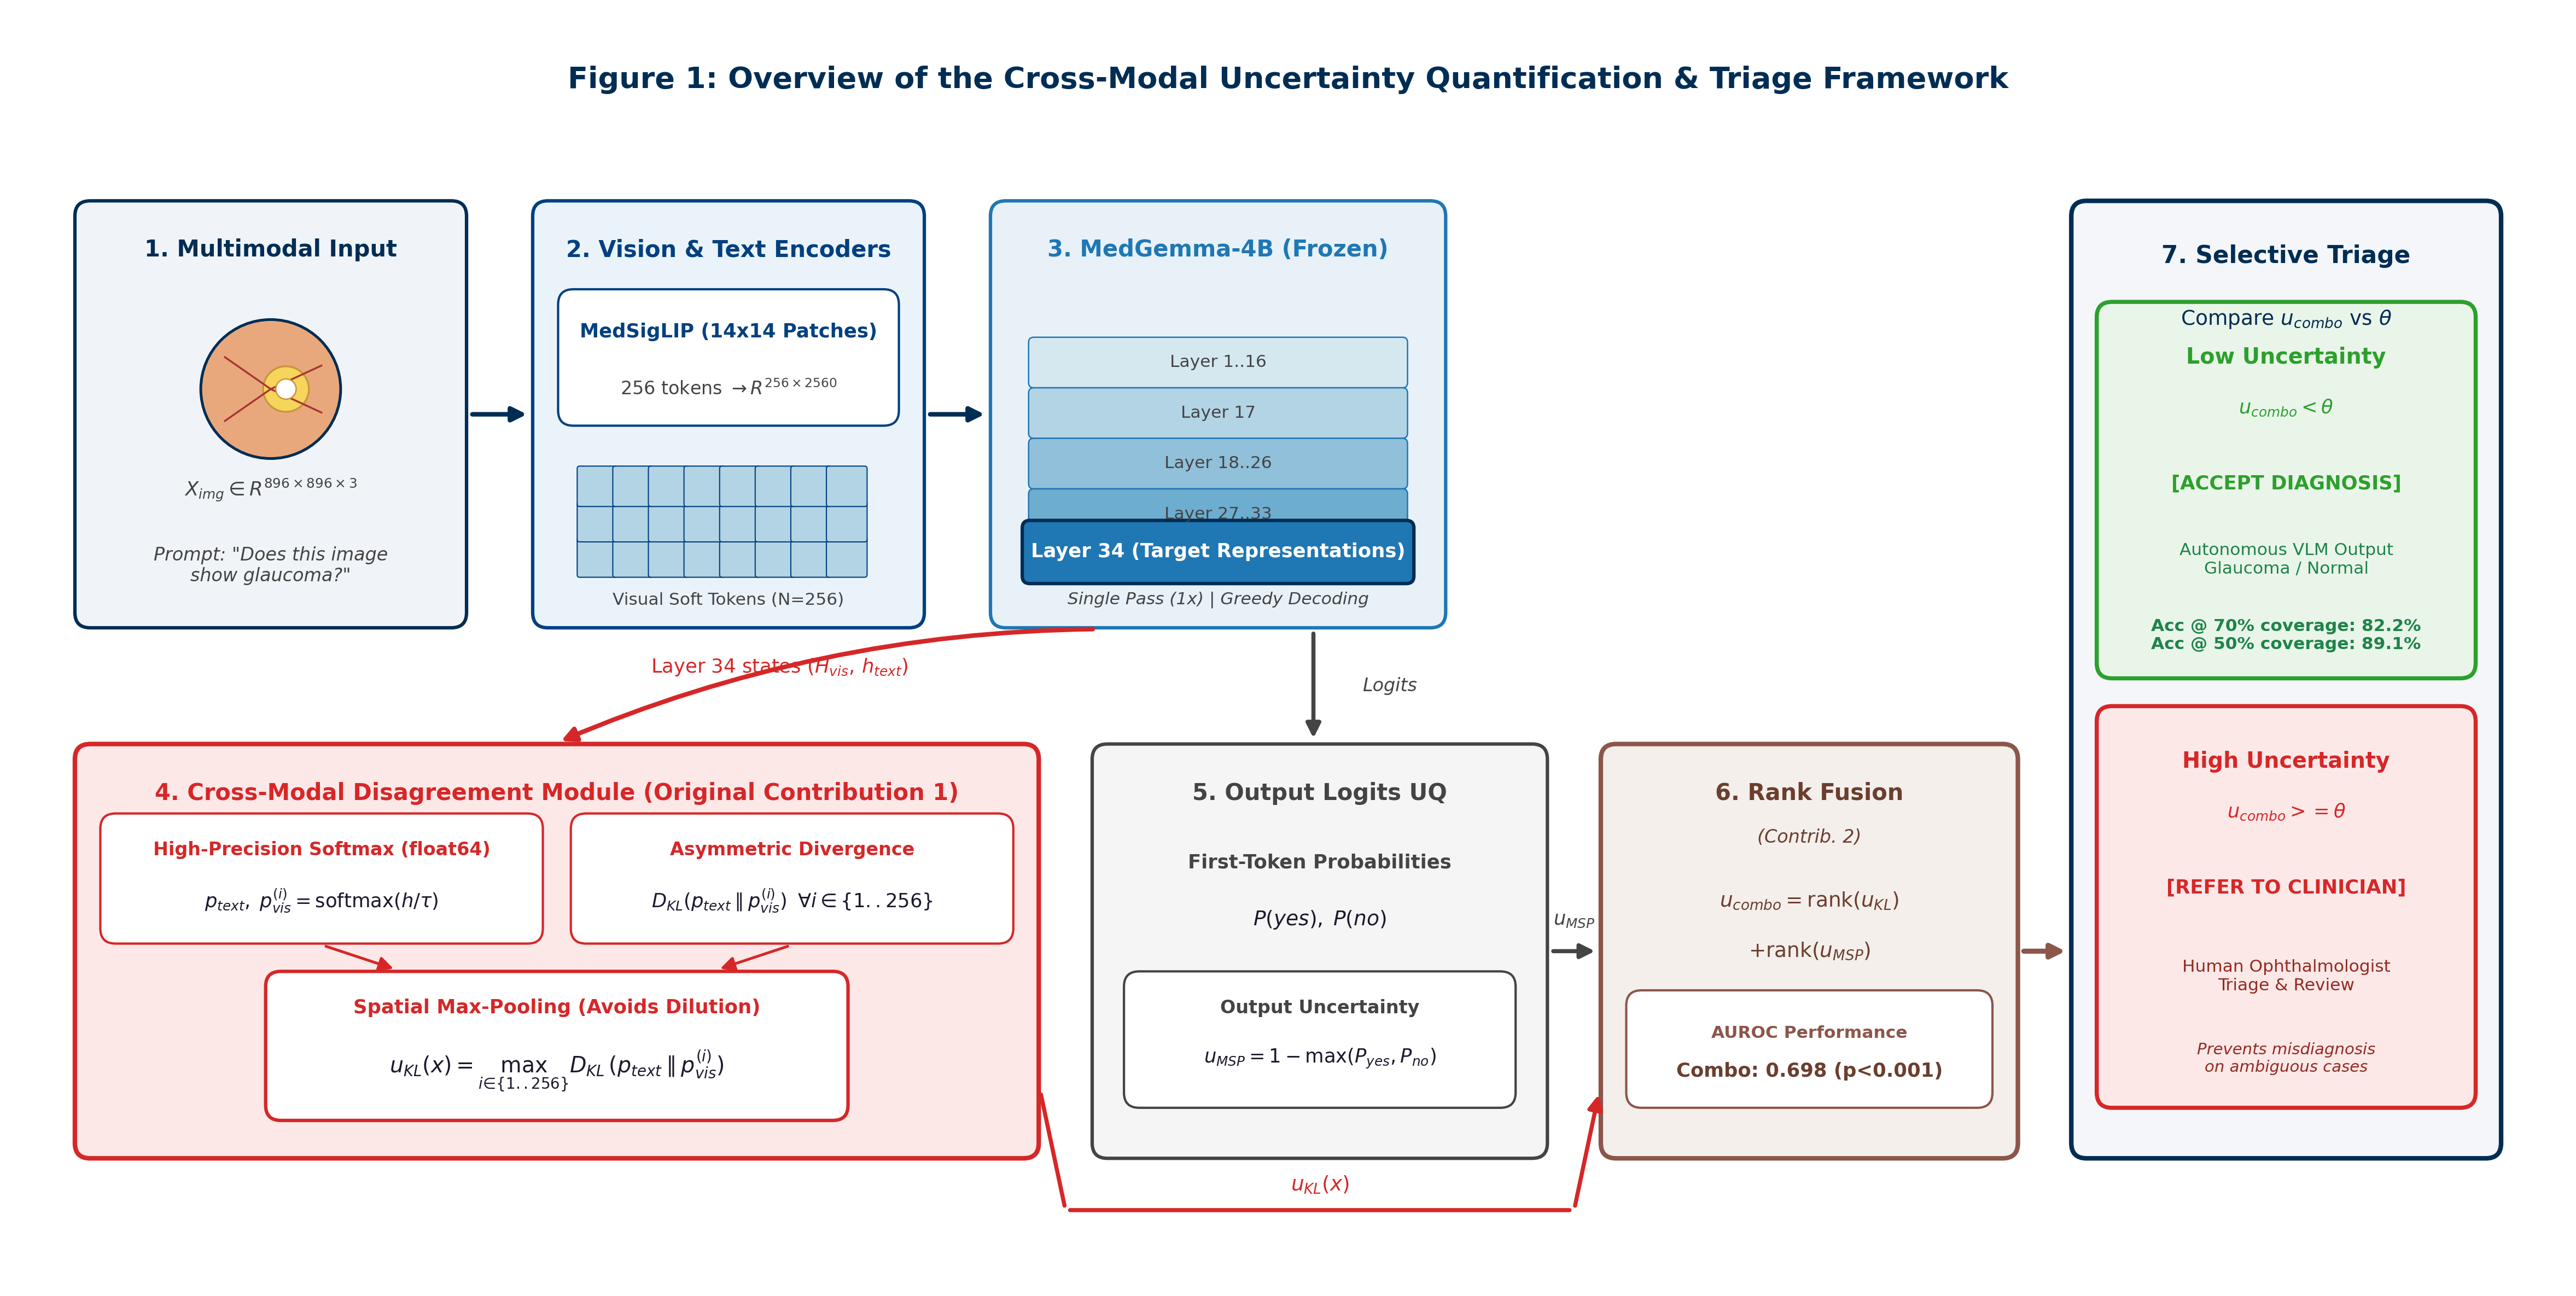
\includegraphics[width=\textwidth]{assets/fig1_pipeline.png}
    \caption{Pipeline del experimento end-to-end: de la imagen de fondo de
    ojo al triage selectivo. El umbral $\theta$ del panel final se define
    como percentil de la cohorte, nunca como valor absoluto de nats
    (Sección~\ref{sec:triage}).}
    \label{fig:pipeline}
\end{figure}

% ============================================================
\section{Resultados obtenidos y su interpretación}
\label{sec:resultados}
% ============================================================

Esta sección presenta los resultados de la Fase 1 con tres preguntas
guía: \emph{qué} se obtuvo, \emph{por qué} se obtuvo así (la forma de
hacerlo) y \emph{qué significa} (la interpretación). Todos los números
provienen de la corrida completa verificada
(\texttt{results/evaluation\_summary.csv}); la fuente canónica y las
figuras están en el repositorio del proyecto.

\subsection{Punto de partida: la accuracy base del modelo y por qué importa}

MedGemma-4B, zero-shot con el prompt P1, clasifica correctamente
\textbf{103 de 129 imágenes: accuracy $= 79.8\%$}. Se equivoca en
\textbf{26 casos} --- esa es la muestra positiva sobre la que se evalúa
toda la UQ. Este valor cae en el escenario ``aceptable'' previsto por el
análisis de riesgo del diseño: el escenario temido era accuracy $> 85\%$
($\sim$13 errores), que habría dejado la evaluación sin poder.

Un dato anticipa todo lo demás: la mediana de $p_{\mathrm{yes}}$ entre
las predicciones afirmativas es $\approx 0.9999$. El modelo \textbf{casi
nunca duda en su output}, lo que explica de antemano por qué los baselines
basados en logits (entropy, MSP) tienen utilidad limitada y por qué hay
que mirar \emph{dentro} del modelo. La interpretación formal: en un modelo
sobreconfiado, el error típico es el \emph{error sobreconfiado} --- baja
entropy de respuesta y, como veremos, alta KL interna simultáneas.

\subsection{Selección de la variante ganadora (solo en train)}
\label{sec:ganadora}

Las 97 variantes se ordenaron por AUROC \textbf{únicamente sobre el split
train} (77 imágenes), excluyendo los poolings oracle. La ganadora se
congeló como hipótesis: \texttt{kl\_t\_v}, capa 34, $\tau = 1$, pooling
\texttt{max} (AUROC train $= 0.728$). La brecha train $\to$ cohorte
($0.728 \to 0.661$) es la esperable ``maldición del ganador'' y se
cuantifica honestamente con Monte Carlo CV (Sección~\ref{sec:generalizacion}).
Que la selección se haga \emph{solo en train} es la pieza anti-optimismo
del protocolo: es lo único que se ``ajusta'' en todo el estudio.

\subsection{Resultado principal (H1): la señal existe y es significativa}
\label{sec:h1}

\begin{figure}[H]
    \centering
    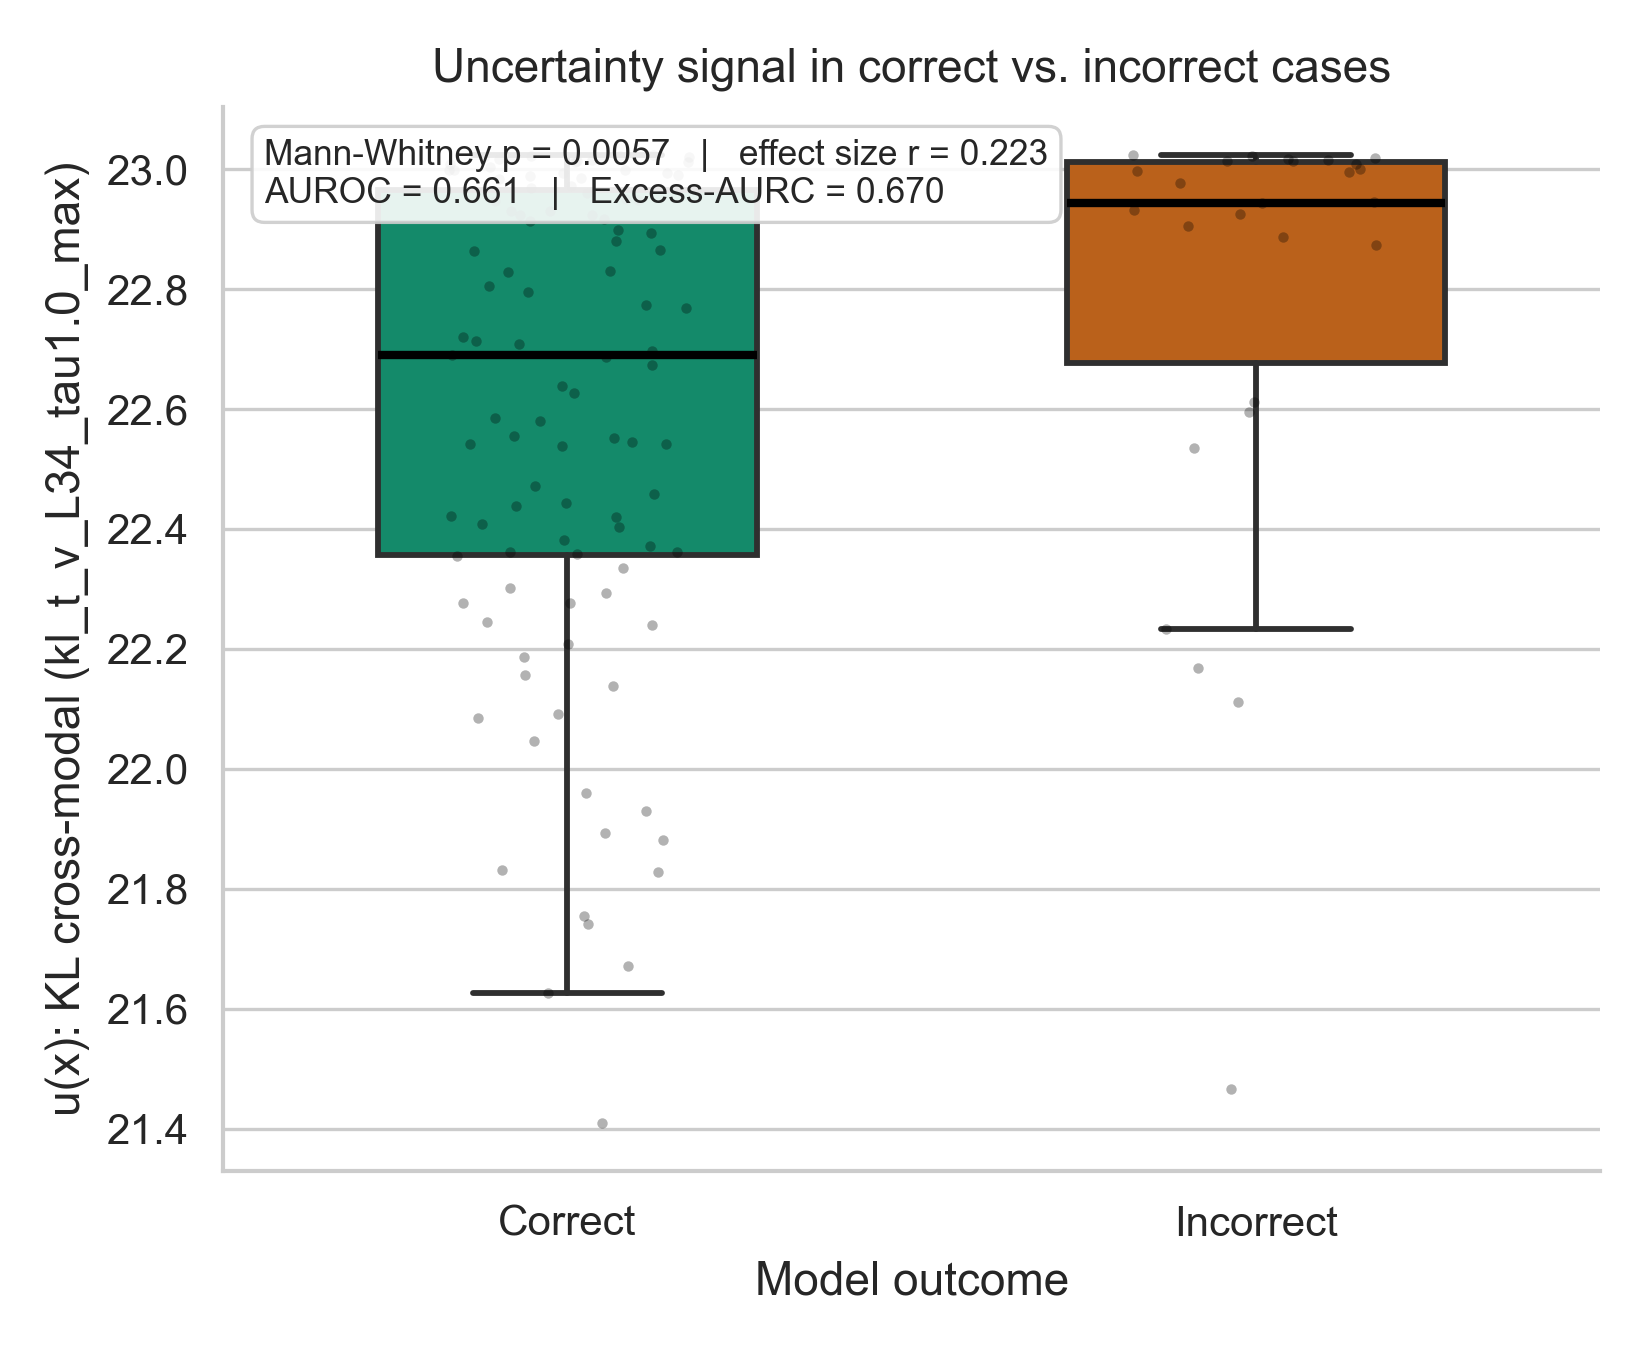
\includegraphics[width=0.72\textwidth]{assets/fig2_boxplot.png}
    \caption{Distribución de la señal KL cross-modal en aciertos vs.\
    errores (P1, $N = 129$). La mediana de los errores es
    significativamente mayor (Mann-Whitney $p = 0.0057$).}
    \label{fig:boxplot}
\end{figure}

La señal KL cross-modal es \textbf{significativamente mayor en los errores
que en los aciertos} (Tabla~\ref{tab:t1}, Figura~\ref{fig:boxplot}):

\begin{table}[H]
\centering
\small
\caption{Tabla T1: resultados principales (P1, $N = 129$, 26 errores).
Accuracy del modelo base: 0.798.}
\label{tab:t1}
\begin{tabular}{lccccccl}
\toprule
\textbf{Señal} & \textbf{AUROC} & \textbf{AUPRC} & \textbf{AURC} & \textbf{Excess-AURC $\downarrow$} & \textbf{Sens@80\%Spec} & \textbf{Costo} \\
\midrule
\textbf{KL cross-modal (ganadora)} & \textbf{0.661} & \textbf{0.329} & \textbf{0.1425} & \textbf{0.670} & \textbf{0.423} & 1$\times$ \\
KL v$\to$t (espejo) & 0.566 & 0.293 & 0.1657 & 0.800 & 0.308 & 1$\times$ \\
Entropy & 0.624 & 0.277 & 0.1543 & 0.736 & 0.385 & 1$\times$ \\
$1 - $ MSP & 0.624 & 0.277 & 0.1543 & 0.736 & 0.385 & 1$\times$ \\
Energy & 0.560 & 0.242 & 0.1830 & 0.896 & 0.308 & 1$\times$ \\
\textbf{rank(KL) + rank($1-$MSP)} & \textbf{0.698} & \textbf{0.375} & \textbf{0.0955} & \textbf{0.407} & 0.308 & 1$\times$ \\
\bottomrule
\end{tabular}
\end{table}

\begin{itemize}[leftmargin=1.4em]
    \item \textbf{Qué:} AUROC $= 0.661$, IC 95\% $[0.522, 0.772]$ (BCa,
    9\,999 remuestreos); Mann-Whitney $p = 0.0057$, effect size
    $r = 0.223$; AUPRC $= 0.329$ $[0.183, 0.478]$.
    \item \textbf{Por qué así:} el AUROC aquí no mide diagnóstico --- mide
    la probabilidad de que un caso mal clasificado tenga mayor $\ux$ que
    uno bien clasificado al escoger una pareja al azar (Mann-Whitney). Con
    26 errores, el AUPRC al azar sería $26/129 \approx 0.202$; el $0.329$
    observado casi lo duplica. El IC se computó por bootstrap BCa porque
    con $N$ pequeño es el método preferido, y se reporta completo aunque
    sea ancho --- es la condición honesta del criterio de éxito.
    \item \textbf{Interpretación:} \textbf{H1 verificada}. El IC excluye
    0.5 (evidencia fuerte) y la estimación puntual cumple la meta de
    diseño ($\geq 0.65$). La lectura teórica: $\KL(\ptext \Vert \pvis)$
    mide cuánto de lo que el modelo está a punto de afirmar no está
    respaldado por su propia representación visual del caso. Cuando el
    modelo ``ve'' algo ambiguo pero ``dice'' algo seguro, la KL sube --- y
    empíricamente eso coincide con el error.
\end{itemize}

\subsection{Comparación con baselines de igual costo (H2)}
\label{sec:h2}

\begin{figure}[H]
    \centering
    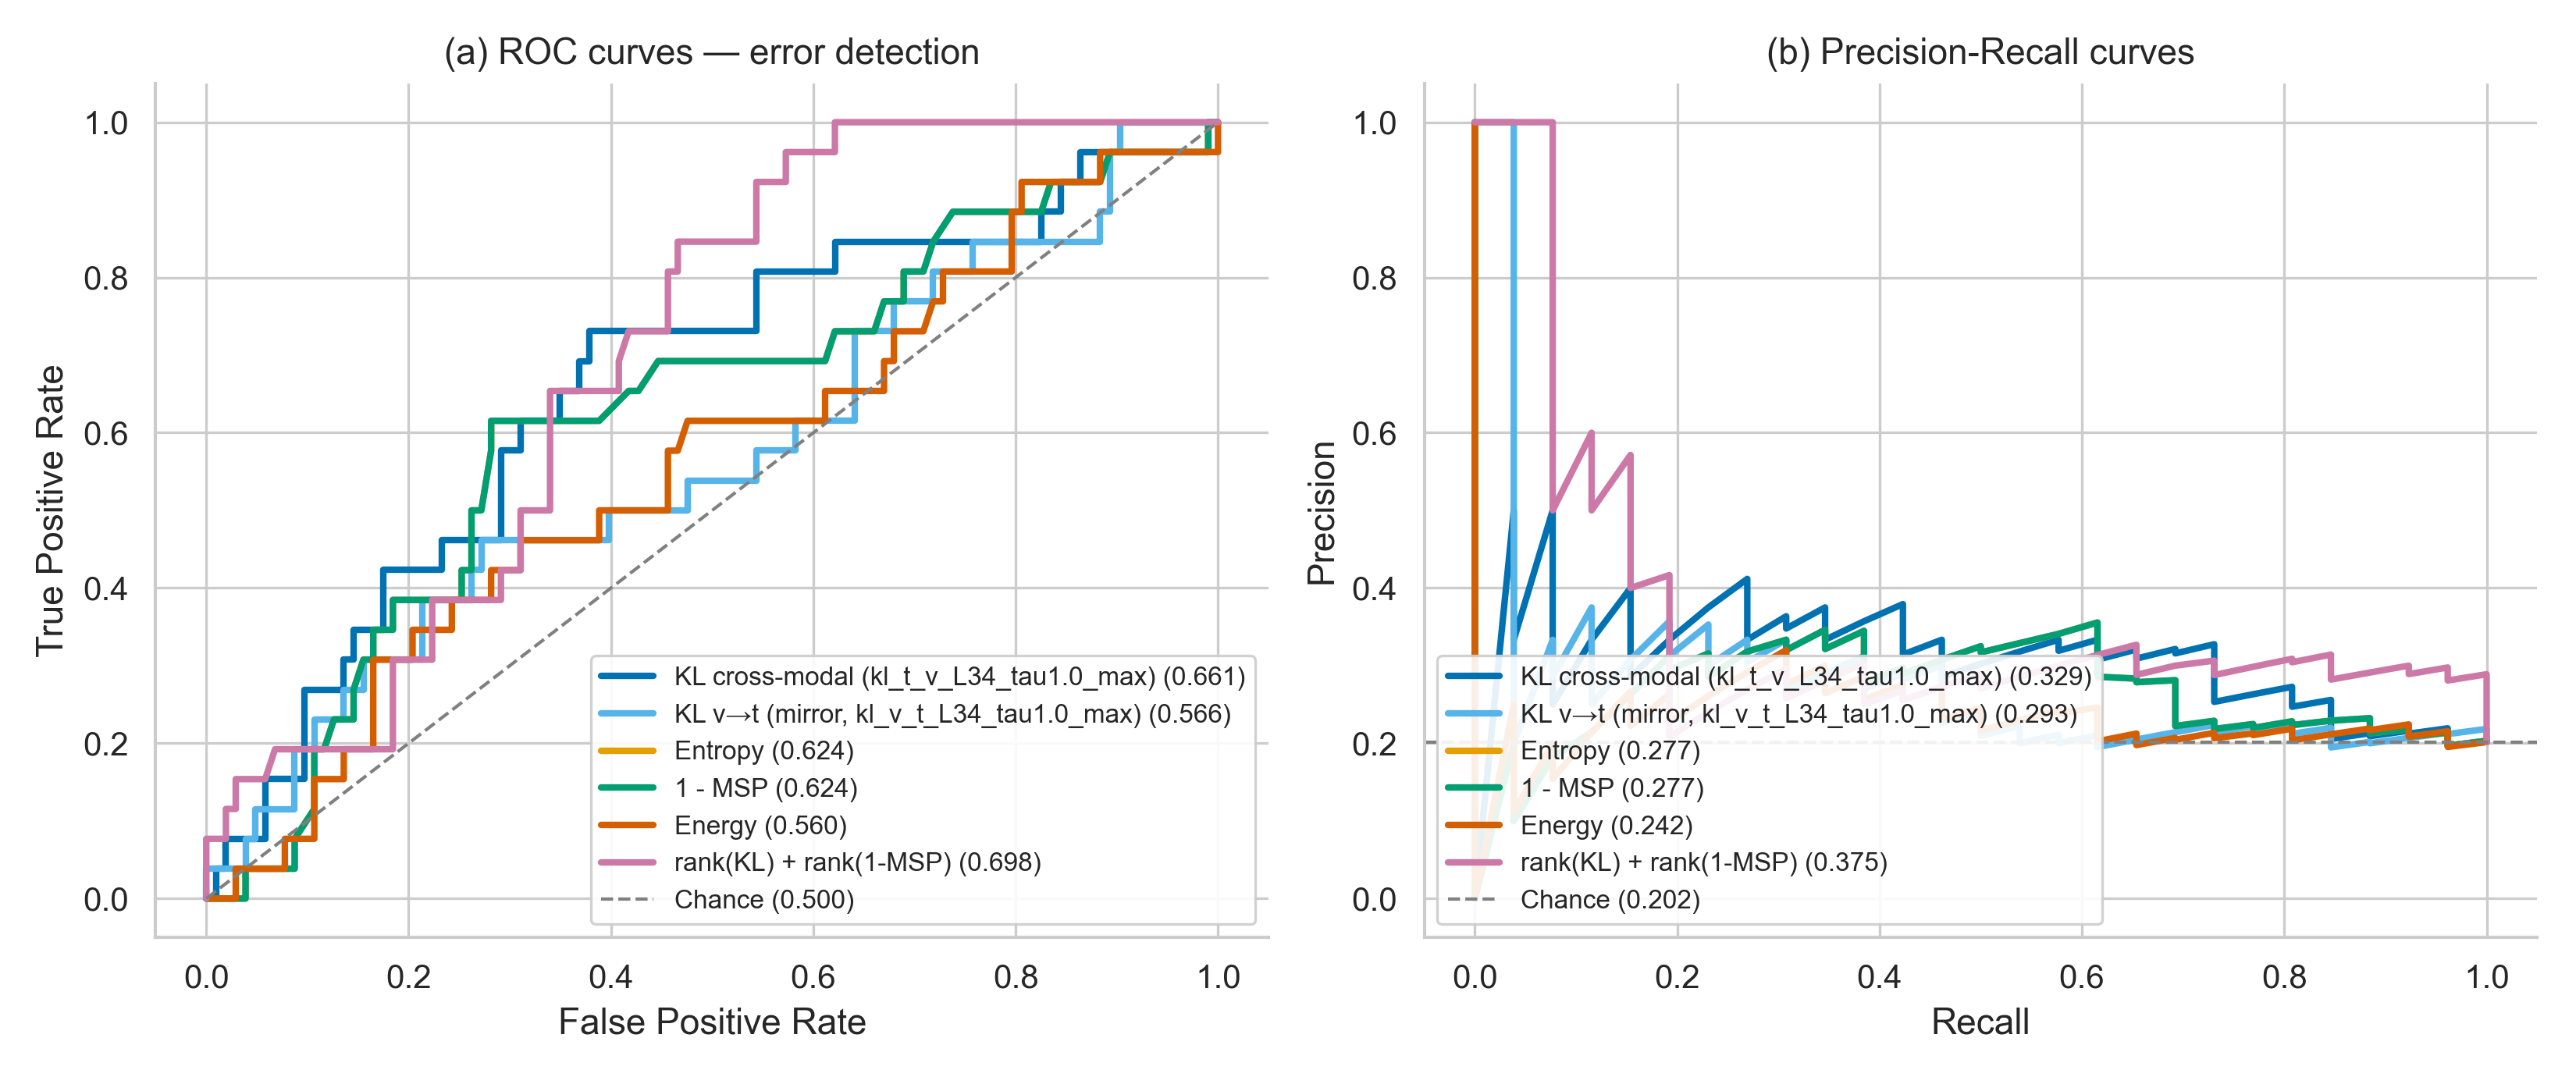
\includegraphics[width=\textwidth]{assets/fig3_roc_pr.png}
    \caption{Curvas ROC y Precision-Recall de todas las señales 1$\times$
    (P1, $N = 129$). La combinación por ranks domina el panel; la KL
    cross-modal supera a los tres baselines de logits.}
    \label{fig:roc}
\end{figure}

\textbf{H2: parcialmente verificada.} La KL supera a los tres baselines
1$\times$ en AUROC ($+0.037$ sobre MSP/entropy, $+0.101$ sobre energy), en
AUPRC y en significancia ($p = 0.0057$ vs.\ $0.0258$ y $0.1745$), pero la
ventaja sobre $1-\mathrm{MSP}$ es modesta. Lectura honesta: la KL no
reemplaza a la confianza del modelo --- \textbf{la complementa}. Las
correlaciones entre señales lo explican (Figura~\ref{fig:corr}):
KL$\perp$MSP $= 0.27$ (complementarias), KL$\perp$energy $= -0.01$
(independientes), entropy $\equiv$ MSP $= 1.00$ (la misma señal con 2
clases), energy--MSP $= 0.84$ (redundantes: por eso energy no aporta).

\begin{figure}[H]
    \centering
    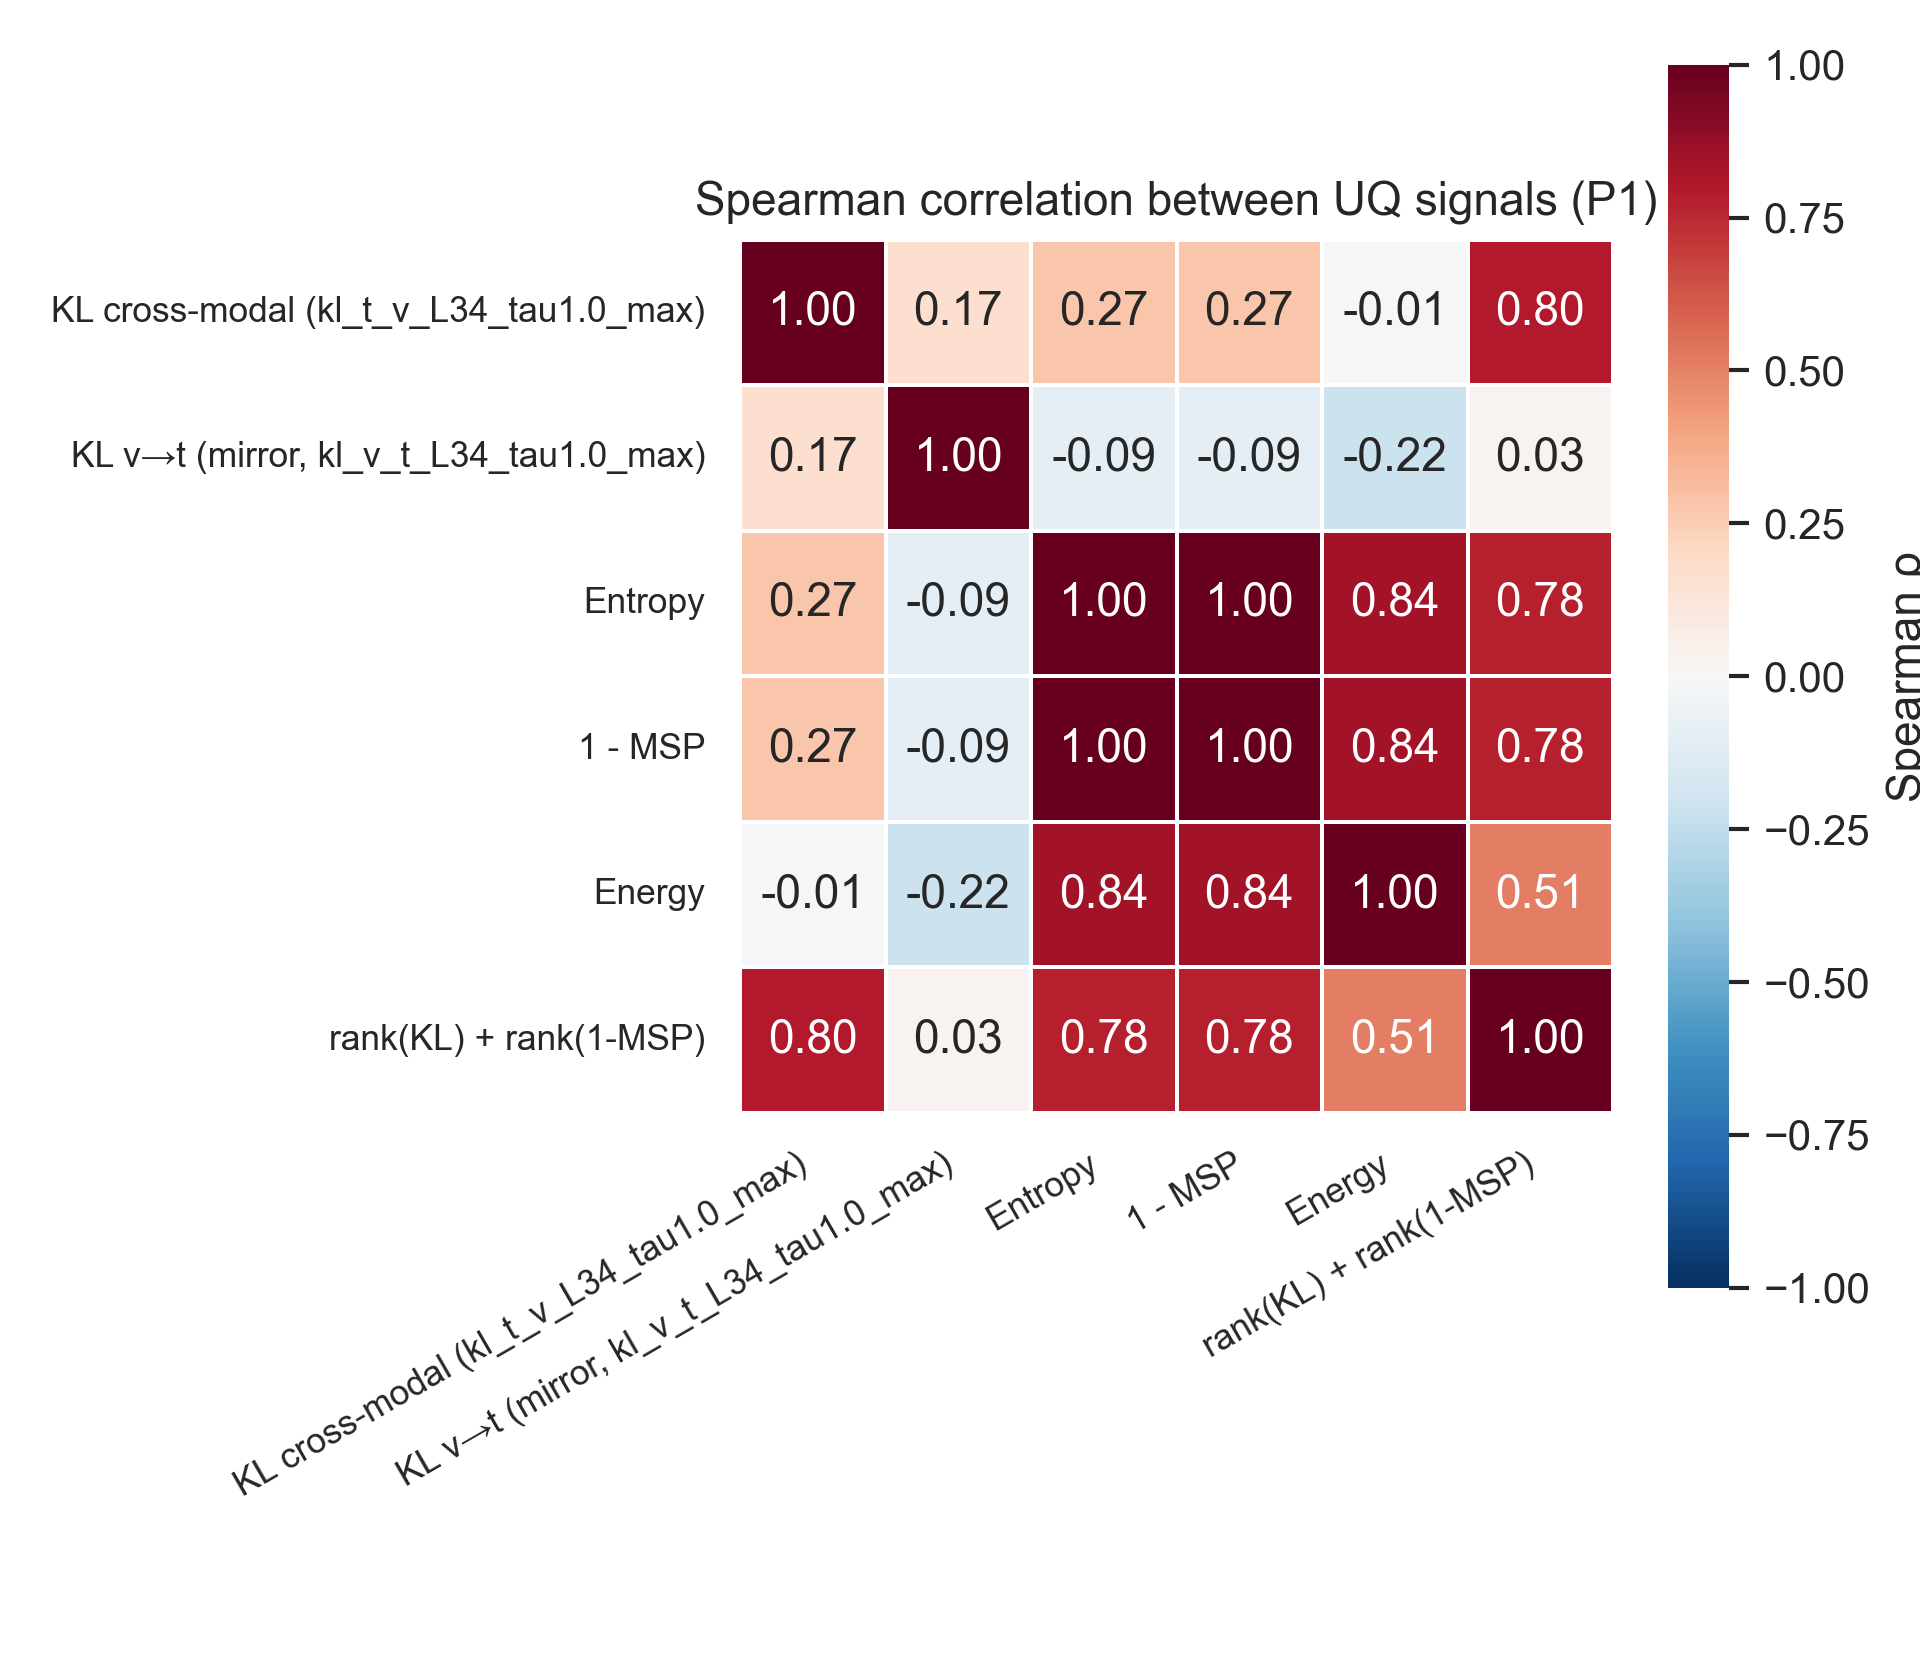
\includegraphics[width=0.62\textwidth]{assets/fig6_correlacion_senales.png}
    \caption{Correlación de Spearman entre señales (P1). La KL es casi
    ortogonal al MSP ($\rho = 0.27$): dos ventanas distintas sobre el
    mismo riesgo.}
    \label{fig:corr}
\end{figure}

\subsection{La señal combinada (H3): contribución original del autor}
\label{sec:h3}

\textbf{Qué:} $u_{\mathrm{combo}}(x) = \mathrm{rank}(\mathrm{KL}) +
\mathrm{rank}(1-\mathrm{MSP})$ alcanza AUROC $= 0.698$ $[0.596, 0.787]$,
$p = 0.00096$; Excess-AURC $= 0.407$ frente a $0.670$ (KL sola) y $0.732$
(MSP solo) --- un \textbf{39\% más cerca del oracle}.

\textbf{Por qué funciona:} con correlación de apenas $0.27$, las dos
señales son ``testigos que vieron cosas distintas'': la KL detecta
errores con respuesta sobreconfiada pero tensión interna imagen$\leftrightarrow$texto;
el MSP detecta errores donde el modelo vaciló sin tensión interna. La suma
de ranks premia a quien es sospechoso para \emph{al menos una} de las dos,
y al operar sobre posiciones es inmune a la incompatibilidad de escalas
(KL $\sim$22--23 nats winsorizados vs.\ MSP en $[0,1]$) que invalida la
suma directa. No hay parámetros que aprender --- a diferencia de una
regresión logística (que probamos y aprendió a ignorar el MSP), esta
combinación \textbf{no puede sobreajustarse}.

\textbf{Advertencia honesta:} con $N = 129$, el IC de la combinación se
solapa con el de la KL sola; se reporta como análisis exploratorio (H3
verificada en ese carácter). La señal primaria del estudio sigue siendo la
KL congelada.

\subsection{Aplicación clínica: triage por percentiles y la zona verde}
\label{sec:triage}

Toda la idea cabe en una imagen mental: \textbf{la fila}. Ordenamos las
129 imágenes de menos a más incierto según $\ux$; el umbral $\theta$ es el
punto donde trazamos la raya: por encima se deriva al oftalmólogo, por
debajo lo responde el modelo solo. $\theta$ se expresa \textbf{como
percentil de la cohorte} (``derivo el 20\% más incierto'' $\Rightarrow$
$\theta =$ percentil 80), nunca como valor absoluto --- los nats no son
portables entre hardware/$\varepsilon$ (Sección~\ref{sec:senal}).

\begin{figure}[H]
    \centering
    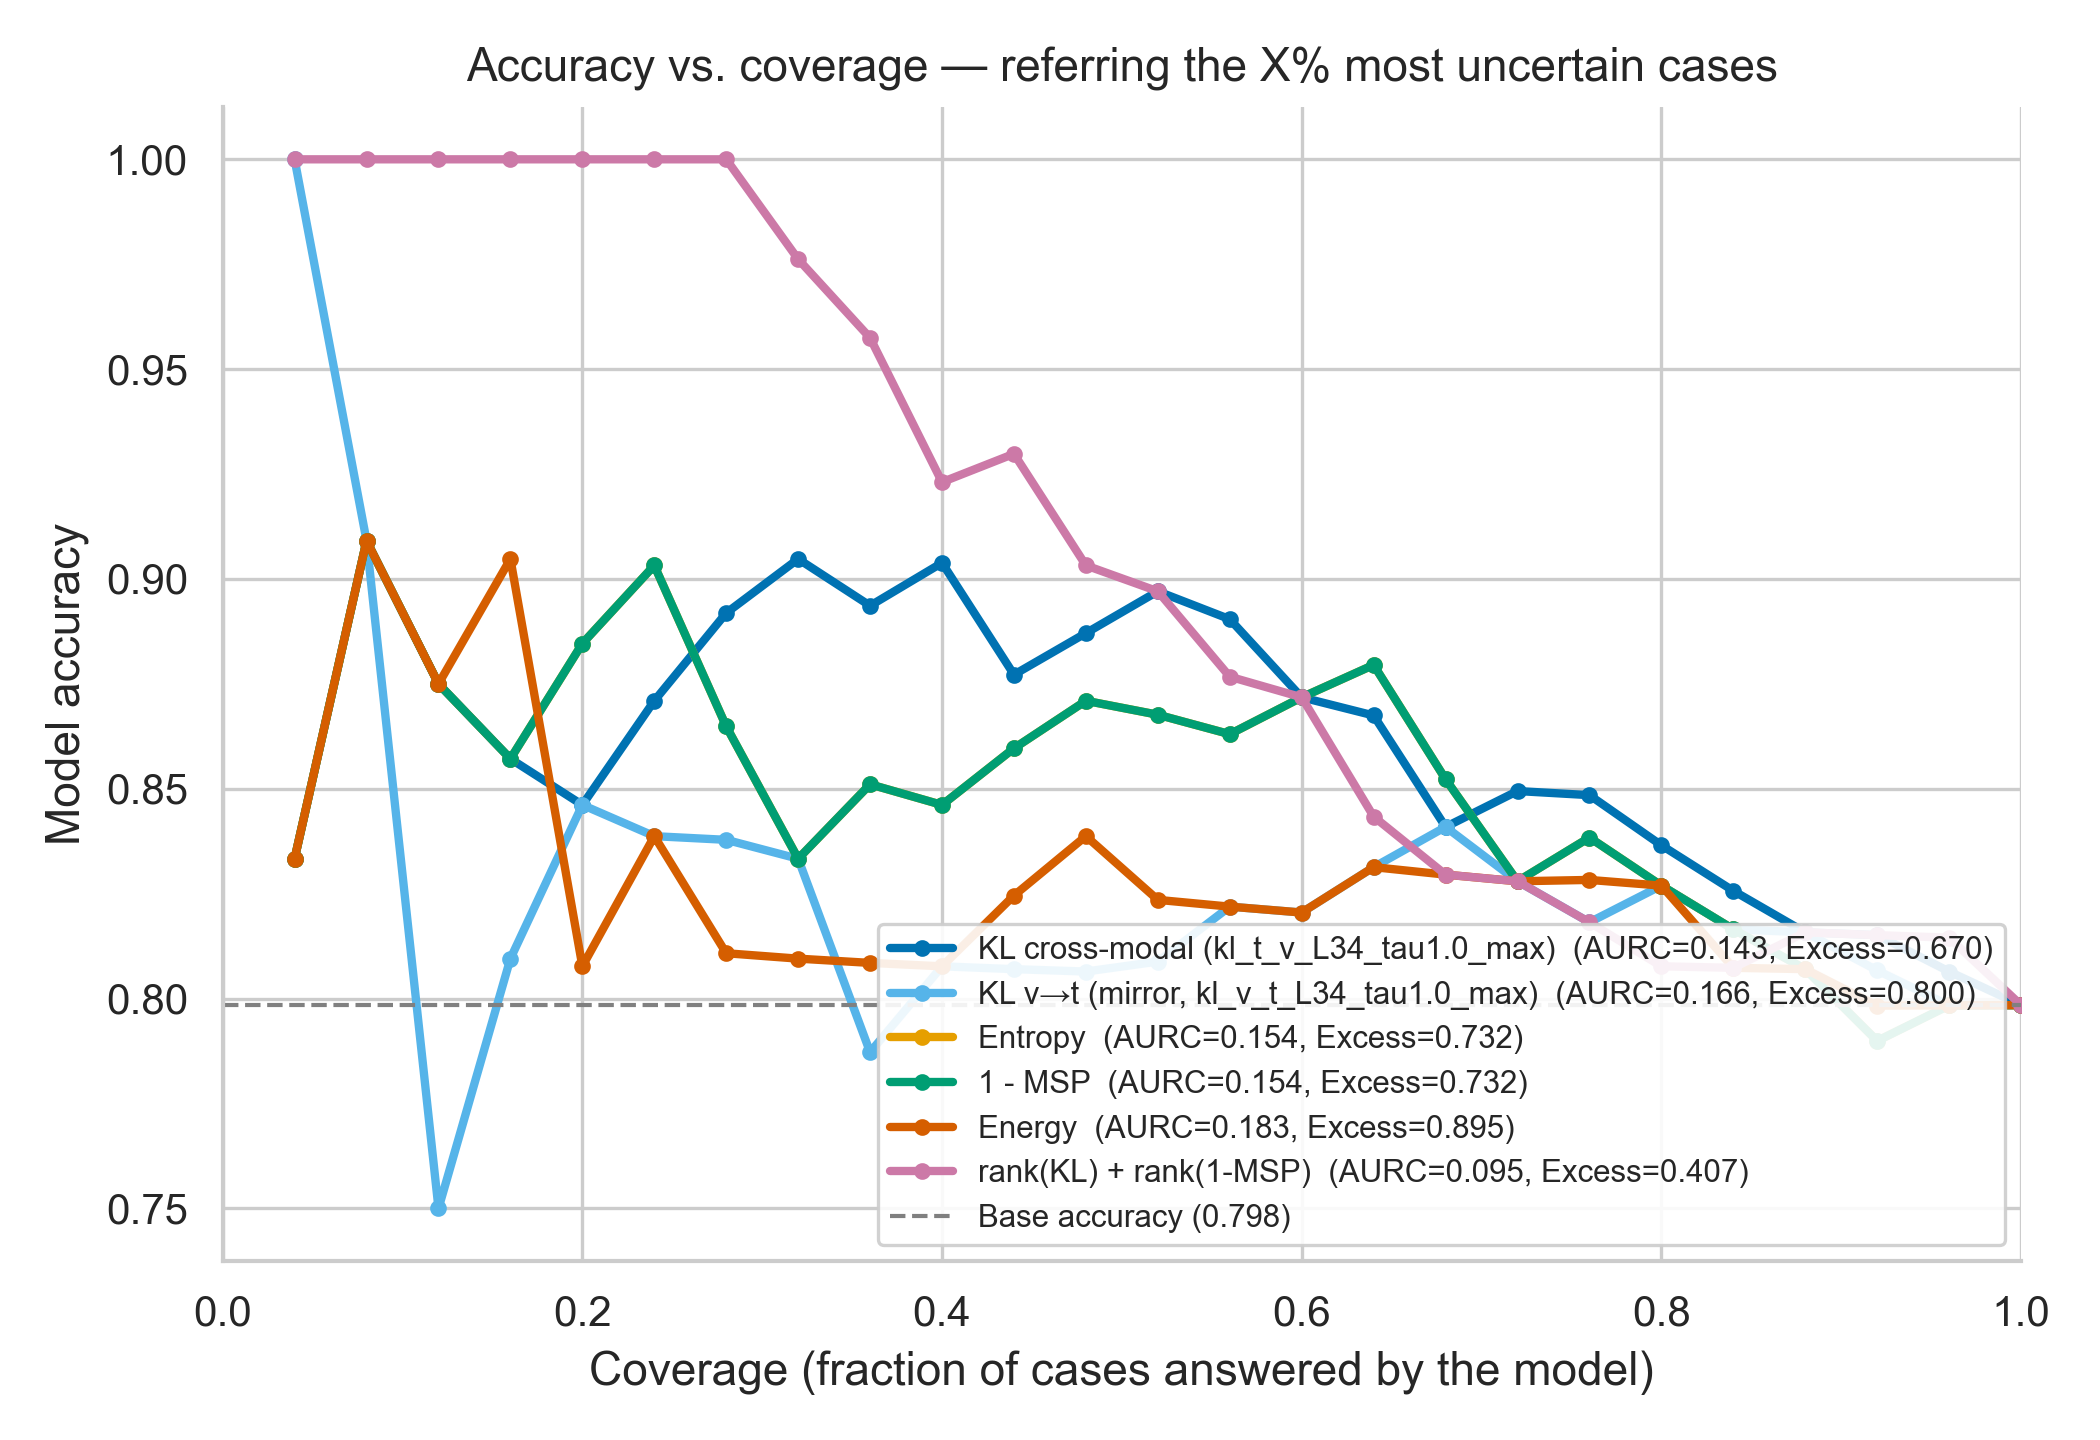
\includegraphics[width=\textwidth]{assets/fig4_accuracy_coverage.png}
    \caption{Accuracy-coverage: accuracy del modelo reteniendo el X\%
    menos incierto. Derivando el 50\% más incierto, la accuracy de lo
    retenido sube de 79.8\% a 89.1\%; a cobertura 30\%, la combinación no
    contiene errores.}
    \label{fig:acccov}
\end{figure}

\begin{table}[H]
\centering
\small
\caption{Decisión de triage (P1, $u_{\mathrm{combo}}$, $N = 129$).}
\label{tab:triage}
\begin{tabular}{lccl}
\toprule
\textbf{Decisión de triage} & $\theta$ \textbf{(punto de corte)} & \textbf{Accuracy en lo retenido} \\
\midrule
Derivar el 10\% más incierto & 1.721 (p90) & 81.9\% \\
Derivar el 20\% & 1.566 (p80) & 81.6\% \\
Derivar el 30\% & 1.318 (p70) & 82.2\% \\
Derivar el 50\% & 0.895 (p50) & \textbf{89.1\%} \\
\textbf{Zona verde} (auto-responder la cola) & 0.686 ($\sim$p30) & \textbf{100\%} (39 casos, en esta cohorte) \\
\bottomrule
\end{tabular}
\end{table}

\paragraph{La zona verde (hallazgo clínico clave).} Verificado
recomputando desde el CSV crudo: los \textbf{39 casos menos inciertos de
la combinación (30.2\% de la cohorte) son todos correctos}; el primer
error aparece en la posición 40 del ranking. \textbf{Advertencias
obligatorias:} (a) la frontera es suave ($\Delta u = 0.004$ entre las
posiciones 39 y 40 --- no es un umbral robusto); (b) la medida es
in-sample: el IC 95\% de la tasa de error en la zona llega hasta
$\sim$7.7\% por la regla de tres (0/39 éxitos).

\paragraph{Interpretación clínica (esquema de 3 zonas).} Auto-responder la
\textbf{cola} ($\sim$30\% de los casos, sin errores en esta cohorte),
derivar la \textbf{cabeza} (los $\sim$7 más inciertos tienen 57\% de
precisión de error --- altísima prioridad) y mandar la \textbf{zona gris
intermedia} al especialista en flujo normal o a pruebas confirmatorias
(OCT, campo visual). ¿Cómo se elige $\theta$ en la práctica? Por
capacidad clínica (cuántos casos puede revisar el especialista), por
especificidad objetivo, o por este esquema de dos umbrales. Por protocolo,
$\theta$ se fija con el split train y se reporta congelado.

\subsection{AURC / Excess-AURC: la segunda métrica que decide}
\label{sec:aurc}

El AURC integra el error del modelo sobre \emph{todos} los niveles de
derivación; el Excess-AURC lo normaliza ($0 =$ oracle, $1 =$ azar). El
AURC \textbf{amplifica el veredicto sobre la combinación}: $0.407$ vs.\
$0.670$ de la KL sola, porque premia acertar en la cabeza de la lista de
derivación, exactamente donde la combinación es fuerte. Concordancia
entre métricas: Spearman(AUROC, Excess-AURC) $= -0.51$ sobre las 97
variantes --- se correlacionan moderadamente pero no son redundantes:
AUROC evalúa el ranking global, AURC los puntos operativos de triage. Las
dos coinciden en elegir a la combinación como \#1.

\subsection{Justificación empírica de la dirección KL}
\label{sec:direccion}

La KL es asimétrica; la elección de dirección fue deliberada y la respuesta
la dieron los datos (P1, $N = 129$): KL(texto$\Vert$imagen) $= 0.661$,
$p = 0.0057$; KL(imagen$\Vert$texto) $= 0.566$, $p = 0.149$ (no
significativa). \textbf{Interpretación:} KL(t$\Vert$v) pondera por donde
el \emph{texto} pone su masa --- mide ``¿el texto afirma lo que la imagen
no respalda?'', la dirección de la \emph{alucinación} $\to$ señal del
error. KL(v$\Vert$t) mide la riqueza trivial imagen$>$texto, casi
constante entre imágenes $\to$ ruido. Detalle fino: el desplazamiento de
medianas es parecido en ambas ($+0.25$ vs.\ $+0.23$), pero el AUROC no,
porque depende del solapamiento completo: en v$\to$t las colas se solapan
mucho más. Una ablación exhaustiva de fusión de direcciones (8 poolings
$\times$ 3 $\tau$ $\times$ 6 esquemas) cerró la puerta final: mezclar
ambas direcciones solo \emph{diluye} la señal. La dirección espejo se
reporta siempre junto a la ganadora como evidencia de que la elección fue
empírica, no arbitraria.

\subsection{Baselines multi-pass: por qué fallan y qué revelan}
\label{sec:multipass}

\subsubsection{Verbalized Confidence (P5, costo 2$\times$)}

\begin{figure}[H]
    \centering
    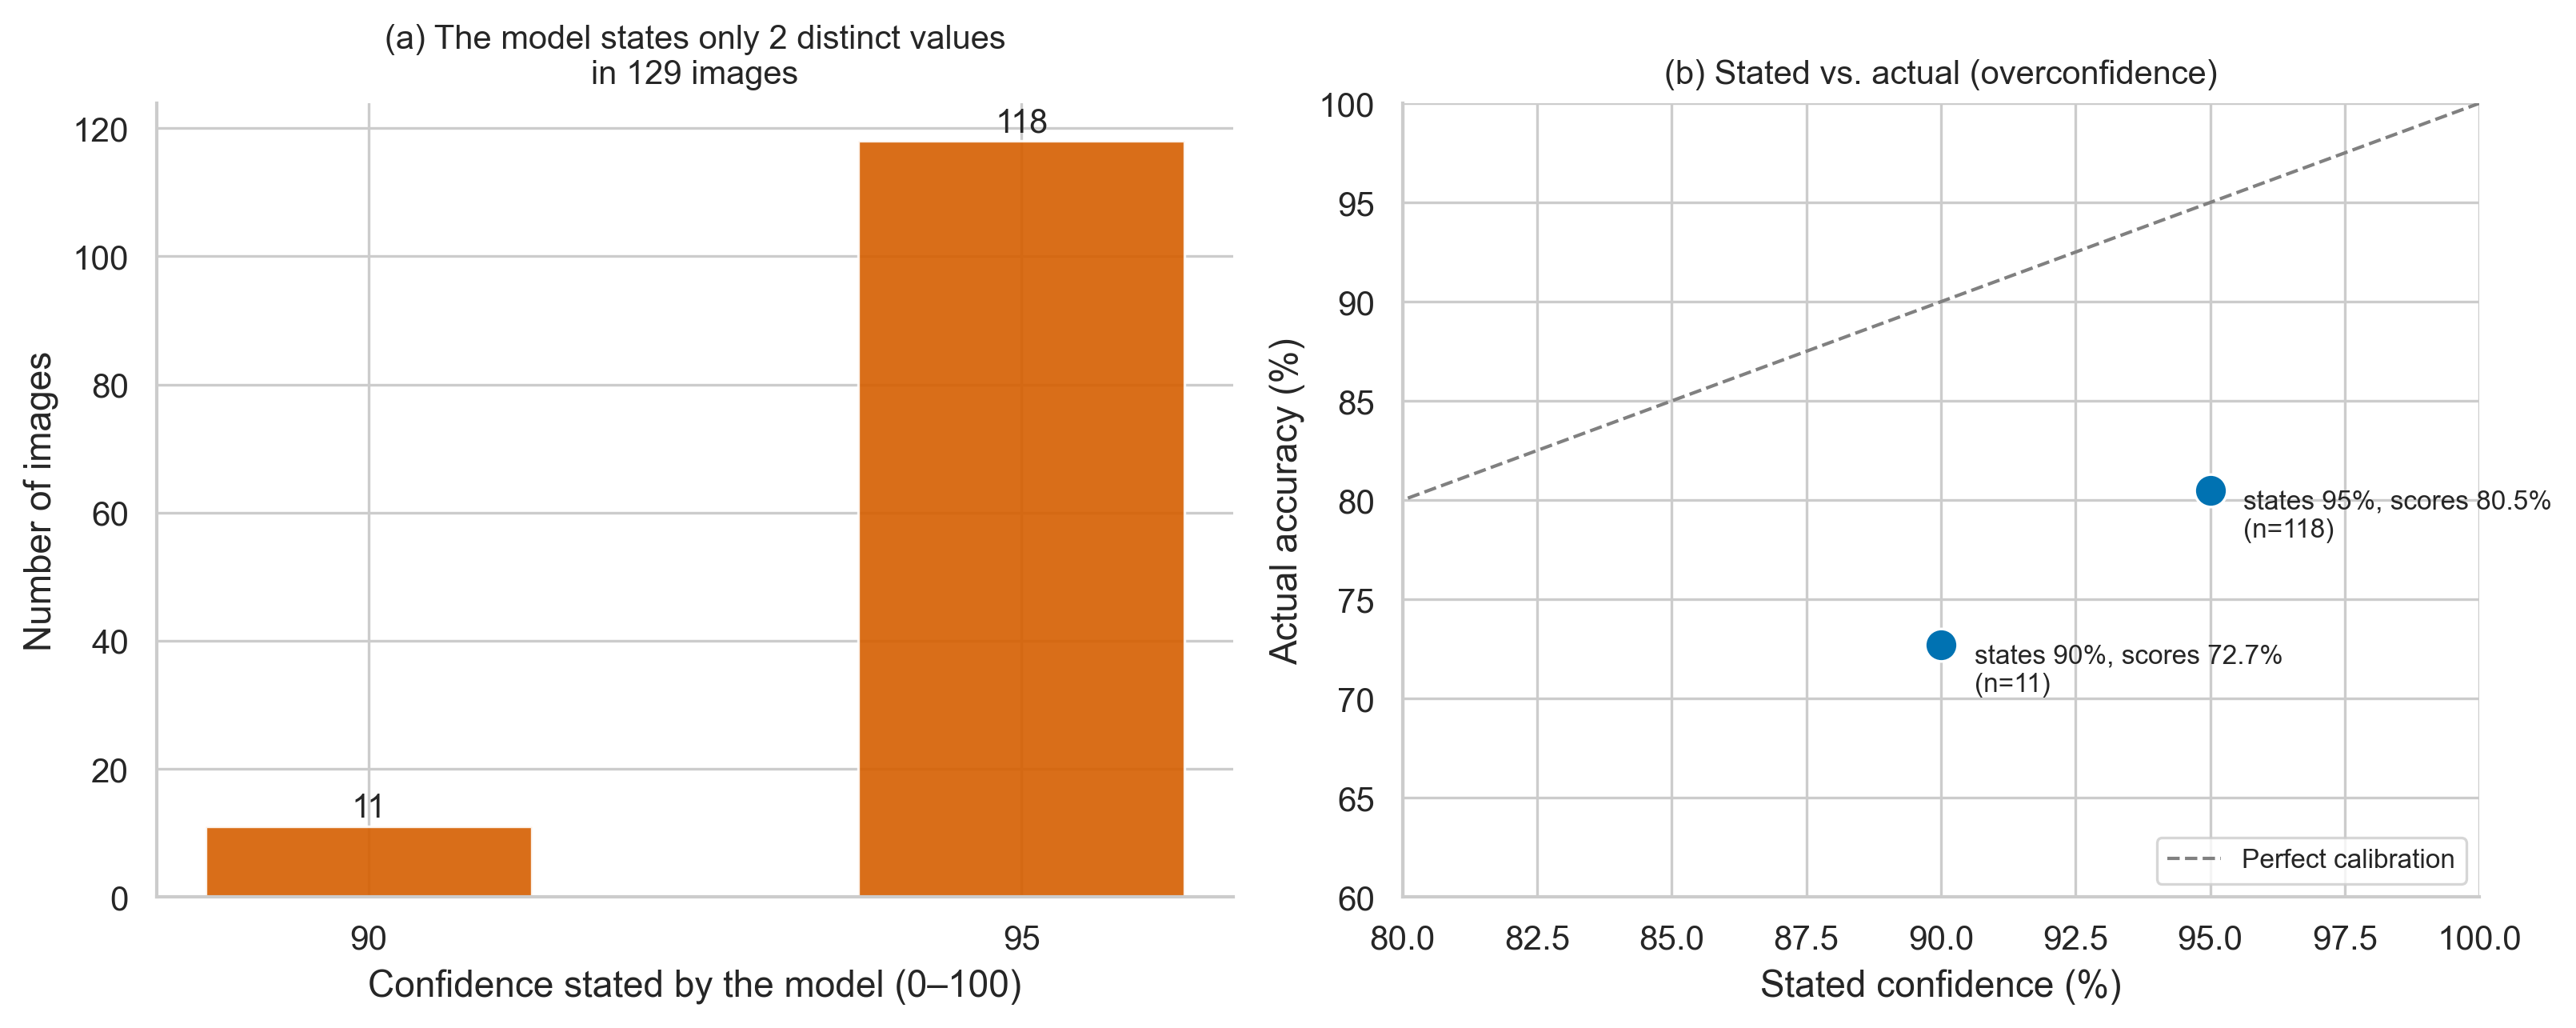
\includegraphics[width=0.75\textwidth]{assets/fig8_verbalized.png}
    \caption{Confianza verbalizada: el modelo solo declara 95 ($n = 118$)
    y 90 ($n = 11$) --- escala degenerada; AUROC $= 0.519 \approx$ azar.}
    \label{fig:verbalized}
\end{figure}

\textbf{Qué:} AUROC $= 0.519$ ($\approx$ azar). \textbf{Por qué:} (a)
degeneración total de la escala --- solo dos valores en 129 respuestas;
una señal con 2 valores no puede rankear 129 casos; (b) sobreconfianza
instruction-tuned --- declara 95\% donde acierta 80.5\%. \textbf{Qué
significa:} ``simplemente preguntarle al modelo'' no funciona; su confianza
declarada no está anclada en su estado interno. Posible limitación
\emph{fundamental} de VLMs instruction-tuned para auto-evaluarse.

\subsubsection{Self-Consistency (SC, costo 10$\times$, $T = 1.5$)}

\textbf{Qué:} mejor señal SC: \texttt{frac\_other} (fracción de muestras
fuera de formato) $\to$ AUROC $= 0.655$, pero $p = 0.054$ (no
significativa); entropía binaria $= 0.573$. \textbf{Por qué:} a $T = 1.5$
la mayoría de las muestras genera tokens \textbf{fuera del formato}
(``based'', ``i'', ``the'') en vez de ``yes''/``no'' --- MedGemma no es
robusto al muestreo estocástico. \textbf{Qué significa:} la inestabilidad
generativa es en sí misma un proxy de incertidumbre, pero más débil que la
KL y 10$\times$ más cara. Nota metodológica: los AUROC del subconjunto SC
(50 imágenes, 12 errores) \textbf{no son comparables} con los de la
cohorte de 129; la comparación justa va etiquetada por separado
(Tabla~\ref{tab:t4}).

\subsubsection{Dominancia Pareto (Tabla T4)}

\begin{table}[H]
\centering
\small
\caption{Tabla T4: costo vs.\ AUROC (conjuntos de evaluación etiquetados
por separado --- nunca mezclados).}
\label{tab:t4}
\begin{tabular}{lclc}
\toprule
\textbf{Método} & \textbf{Costo} & \textbf{AUROC} & \textbf{Conjunto} \\
\midrule
rank(KL)+rank($1-$MSP) & 1$\times$ & 0.698 & 129 \\
KL cross-modal (nuestra) & 1$\times$ & 0.661 & 129 \\
$1-$MSP & 1$\times$ & 0.624 & 129 \\
Energy & 1$\times$ & 0.560 & 129 \\
Verbalized Confidence & 2$\times$ & 0.519 & 129 \\
\midrule
\textbf{KL cross-modal (nuestra)} & \textbf{1$\times$} & \textbf{0.781} & 50 (subconjunto SC) \\
rank(KL)+rank($1-$MSP) & 1$\times$ & 0.731 & 50 (SC) \\
SC frac\_other & 10$\times$ & 0.655 & 50 (SC) \\
$1-$MSP & 1$\times$ & 0.573 & 50 (SC) \\
SC entropía binaria & 10$\times$ & 0.573 & 50 (SC) \\
\bottomrule
\end{tabular}
\end{table}

\begin{figure}[H]
    \centering
    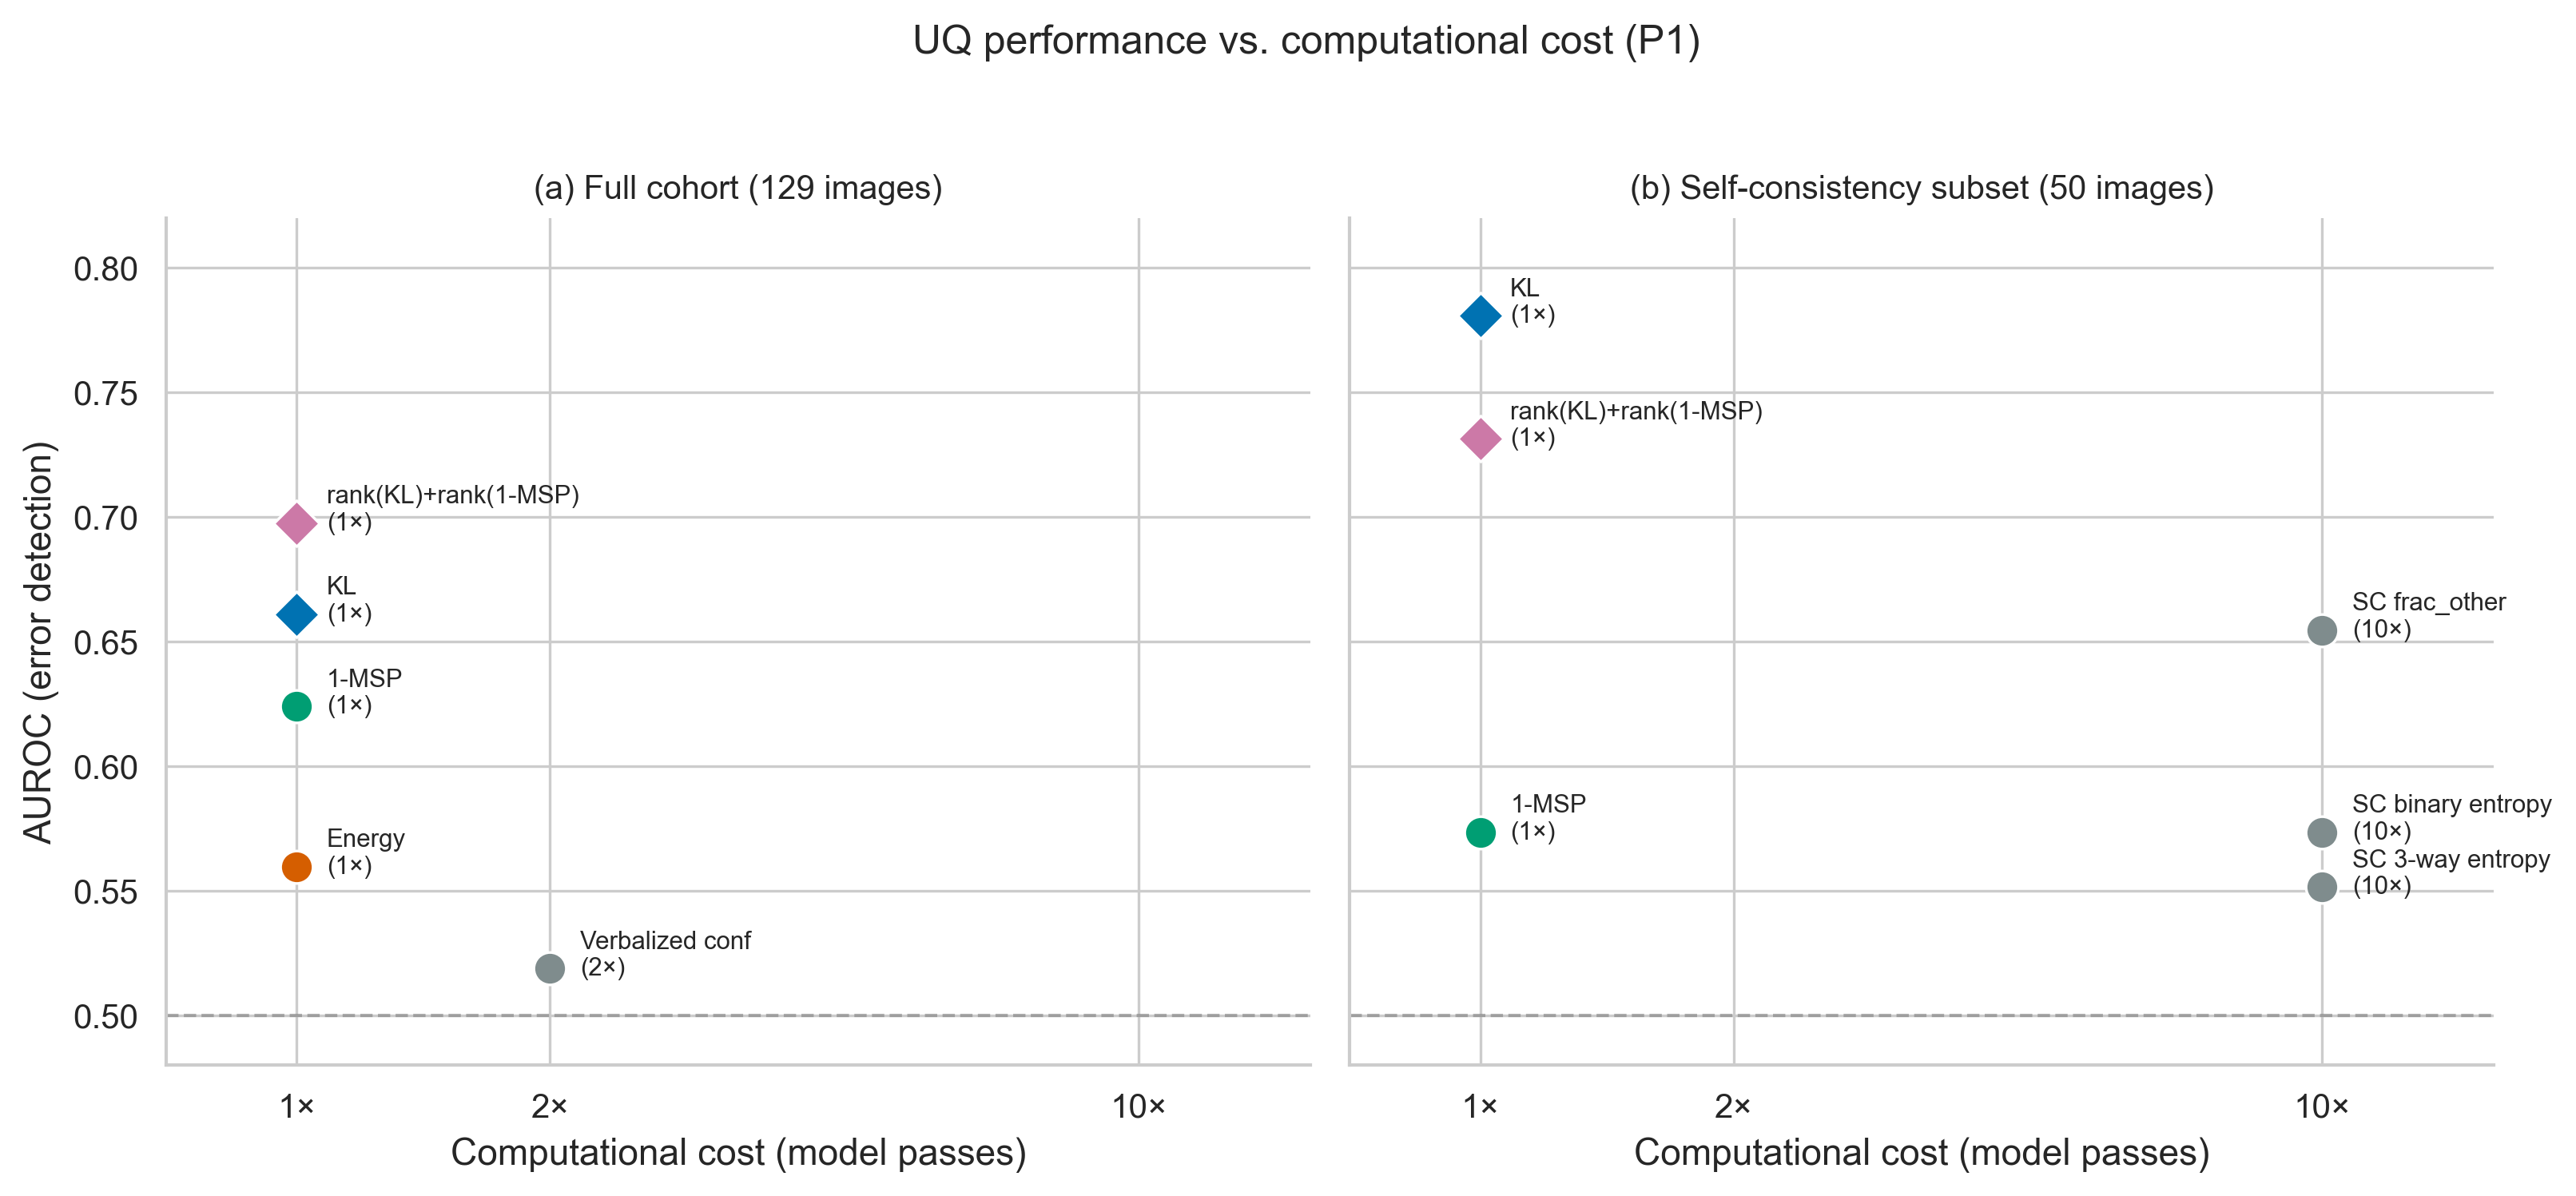
\includegraphics[width=0.8\textwidth]{assets/fig7_costo_vs_auroc.png}
    \caption{Costo computacional vs.\ AUROC: la KL cross-modal (1$\times$)
    domina en el frente de Pareto a todos los baselines multi-pass.}
    \label{fig:pareto}
\end{figure}

\textbf{Resultado central:} en comparación justa sobre las mismas 50
imágenes, KL (1$\times$) $= 0.781$ vs.\ SC frac\_other (10$\times$) $=
0.655$: nuestra señal \textbf{domina a todos los baselines multi-pass con
10$\times$ menos cómputo}. La lección conjunta: la señal cross-modal
(interna) captura información que la señal de output (logits, texto
generado, confianza declarada) \emph{no puede ver}, porque el desacuerdo
entre modalidades ocurre \textbf{antes de la generación} --- en los hidden
states, no en lo que el modelo ``dice''.

\subsection{Ablaciones: por qué la configuración ganadora es la ganadora}
\label{sec:ablaciones}

\begin{itemize}[leftmargin=1.4em]
    \item \textbf{Tipo de divergencia.} kl\_t\_v ($0.661$) $>$ JSD
    ($0.572$, saturada en su techo $\ln 2$ por la brecha modal: no puede
    rankear) $>$ coseno ($0.51$--$0.57$, dominado por massive activations)
    $>$ kl\_prompt ($0.483$, \emph{peor que azar}: control negativo
    valioso --- la señal vive en la \emph{respuesta} que el modelo está a
    punto de emitir, no en la pregunta).
    \item \textbf{Pooling.} \texttt{max} ($0.661$) $\gg$ \texttt{mean}
    ($0.516$: dilución espacial confirmada) $>$ poolings por atención
    (\texttt{attn} $0.479$, \texttt{rollout} $0.533$, \texttt{headspec}
    $0.469$: la atención de un modelo frozen zero-shot no está alineada
    con la tarea; los heatmaps muestran atención difusa por el fondo).
    \textbf{Hallazgo contraintuitivo:} el oracle \texttt{roi} (máscara
    exacta del disco) \emph{empeora} la señal en la corrida completa
    ($0.349$, $n = 69$) --- el $0.889$ del piloto era artefacto de muestra
    pequeña. Hipótesis: la tensión informativa no vive solo en el disco;
    el contexto global del fundus (que \texttt{max} sí ve) aporta a la
    señal.
    \item \textbf{Temperatura.} $\tau = 1$ gana siempre ($0.661$ vs.\
    $0.578$ y $0.525$ con $\tau = 2, 4$): aplastar la softmax homogeniza
    las distribuciones y desaparece la estructura que distingue ``texto
    anclado'' de ``texto alucinado''. El diseño probó $\tau > 1$ como
    remedio a la brecha modal; los datos dijeron que la brecha \emph{es}
    la señal, no el problema.
    \item \textbf{Capa.} Solo la capa 34 produce señal útil: en las capas
    17/26 la KL colapsa (las representaciones aún no han formado la
    decisión). Conecta con la literatura de probing y abre el future work
    de barrido fino 27--34 y early-exit.
    \item \textbf{Prompt.} P1 (ingenuo) $>$ P4 (experto) en todo
    ($0.661$ vs.\ $0.614$; combinación $0.698$ vs.\ $0.654$).
    Interpretación de trabajo: el system prompt de experto ``alinea'' las
    representaciones, homogenizando el estado textual y \emph{reduciendo
    el desacuerdo cross-modal} que es nuestra señal. Paradoja útil: hacer
    el prompt más ``profesional'' hace al modelo algo mejor calibrado en
    output (MSP sube) pero menos transparente internamente (KL baja).
\end{itemize}

\subsection{Generalización honesta: val+test y Monte Carlo CV}
\label{sec:generalizacion}

\begin{table}[H]
\centering
\small
\caption{Estimación de generalización (AUROC).}
\label{tab:generalizacion}
\begin{tabular}{lc}
\toprule
\textbf{Evaluación} & \textbf{AUROC} \\
\midrule
val+test oficial (52 imgs, \textbf{solo 6 errores}) & 0.569 [0.200, 0.938] --- sin poder \\
Monte Carlo CV (200 splits), \textbf{selección anidada} & $0.581 \pm 0.116$ \\
Monte Carlo CV, \textbf{variante congelada} & $0.660 \pm 0.071$ \\
Combinación por ranks, KL congelada & $0.698 \pm 0.062$ \\
Combinación por ranks, re-selección anidada & $0.648 \pm 0.087$ \\
\bottomrule
\end{tabular}
\end{table}

\textbf{Discusión honesta:} el desempeño real de la KL sola en pacientes
nuevos está probablemente en $\sim$0.58--0.66 --- el $0.661$ de la cohorte
completa es optimista por la maldición del ganador. La \textbf{combinación
es la señal más robusta entre splits}: mantiene 0.648--0.698 y su std es
la menor en el régimen congelado. La confirmación en val+test oficial es
estadísticamente vacía (IC $[0.200, 0.938]$ con 6 errores) y se reporta
solo por completitud del protocolo.

\subsection{Calibración de la señal (evidencia secundaria, estilo FUSE §5.2)}
\label{sec:calibracion}

Además de discriminar (ranking), una señal de triage idealmente debería
estar \textbf{calibrada}: a mayor $\ux$, mayor probabilidad empírica de
error. Protocolo: Platt scaling ajustado \textbf{solo en train} y aplicado
congelado; ECE con 10 bins equiprobables ($\sim$13 obs/bin); correlaciones
Pearson/Spearman; Brier; IC bootstrap.

\begin{table}[H]
\centering
\small
\caption{Tabla T5: discriminación + calibración lado a lado (P1, $N = 129$).}
\label{tab:t5}
\begin{tabular}{lccccccc}
\toprule
\textbf{Señal} & \textbf{AUROC} & \textbf{TPR@FPR10\%} & \textbf{TPR@FPR20\%} & \textbf{ECE $\downarrow$} & \textbf{Cal. Pearson} & \textbf{Cal. Spearman} & \textbf{Brier} \\
\midrule
\textbf{KL cross-modal} & \textbf{0.661} & \textbf{0.269} & \textbf{0.423} & \textbf{0.087} & \textbf{0.748} & \textbf{0.789} & \textbf{0.159} \\
KL v$\to$t (espejo) & 0.566 & 0.192 & 0.308 & 0.074 & 0.283 & 0.532 & 0.164 \\
Entropy / $1-$MSP & 0.624 & 0.102 & 0.385 & 0.116 & 0.094 & 0.612 & 0.164 \\
Energy & 0.560 & 0.077 & 0.308 & 0.111 & 0.269 & 0.181 & 0.164 \\
rank(KL)+rank($1-$MSP) & \textbf{0.698} & 0.192 & 0.308 & 0.145 & 0.549 & 0.656 & \textbf{0.159} \\
\bottomrule
\end{tabular}
\end{table}

\begin{figure}[H]
    \centering
    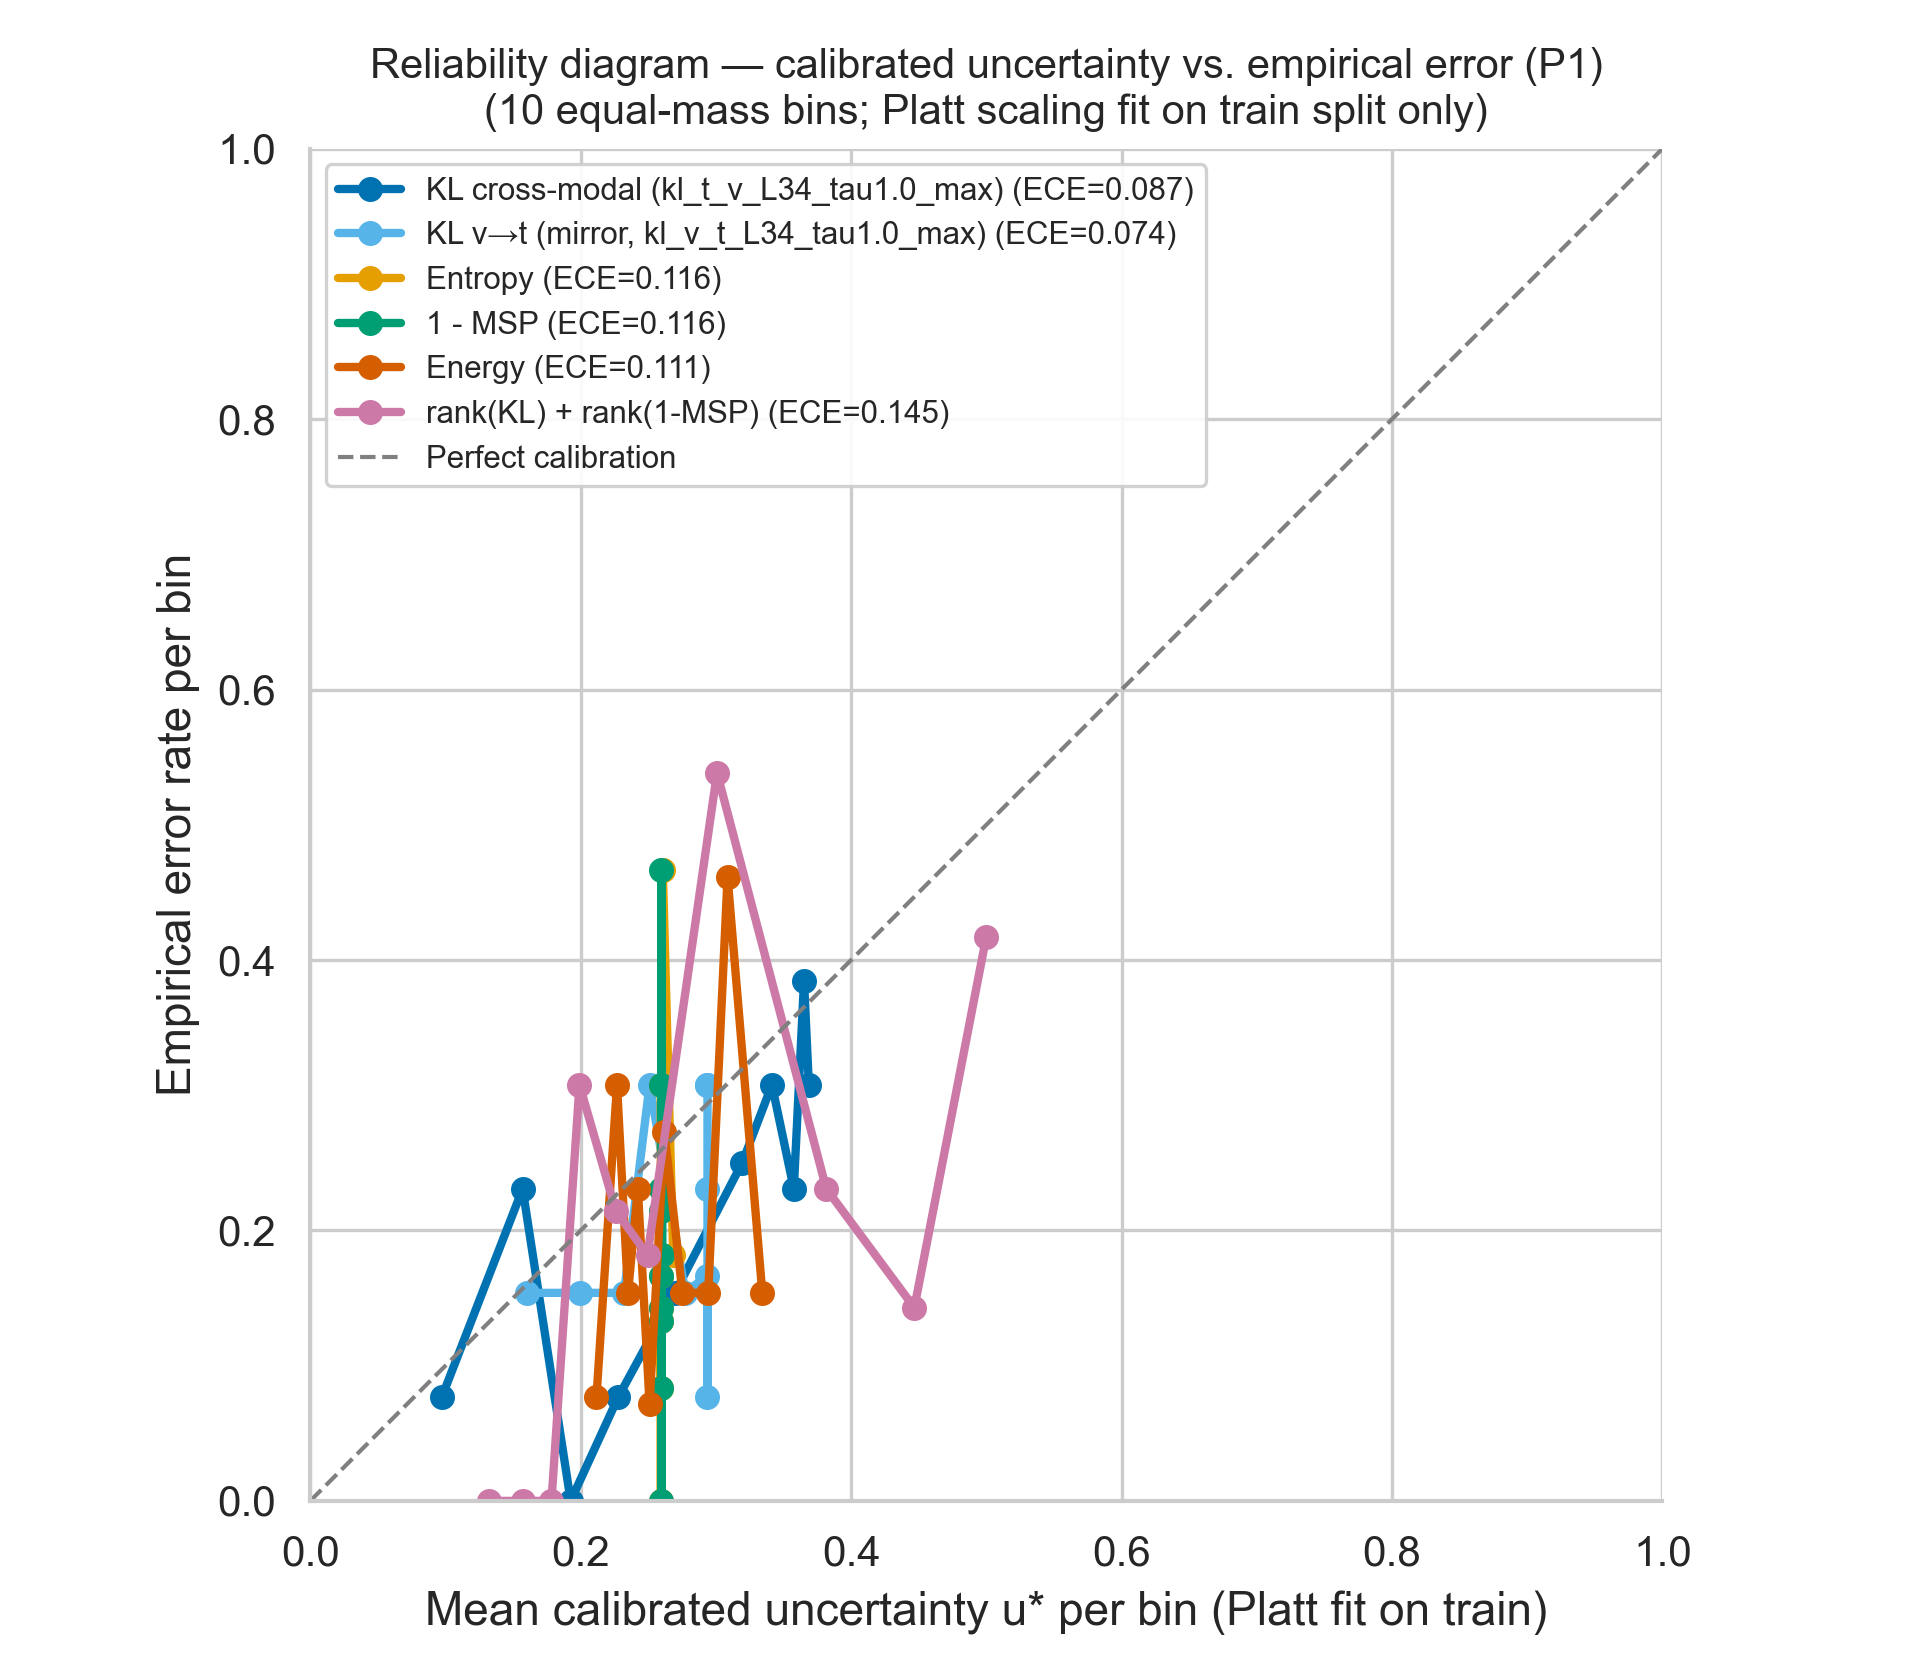
\includegraphics[width=0.7\textwidth]{assets/fig10_reliability.png}
    \caption{Reliability diagram de calibración (Platt ajustado en train,
    bins equiprobables).}
    \label{fig:reliability}
\end{figure}

\textbf{Lectura:} la KL cross-modal es la \textbf{mejor calibrada entre
las señales 1$\times$ discriminativas} (ECE $0.087$; correlaciones
$0.748/0.789$ --- las más altas con diferencia). La \textbf{combinación
discrimina más pero calibra peor} (ECE $0.145$): trade-off real a
declarar --- para triage por ranking se usa la combinación; para
probabilidad de error interpretable, la KL sola. Entropy/MSP tienen
correlaciones de calibración casi nulas ($0.02$--$0.09$): con
$p_{\mathrm{yes}}$ saturada, la confianza de salida no dice nada sobre la
probabilidad de error. \textbf{Advertencias honestas:} con $\sim$13
obs/bin el ECE es ruidoso; Platt es monótona por construcción
(correlaciones altas no prueban calibración por sí solas: la evidencia
principal es ECE + reliability diagram); la calibración \textbf{no} entra
en H1--H4: es análisis complementario post-hoc.

\subsection{Análisis cualitativo: los cuatro cuadrantes}
\label{sec:cuadrantes}

\begin{figure}[H]
    \centering
    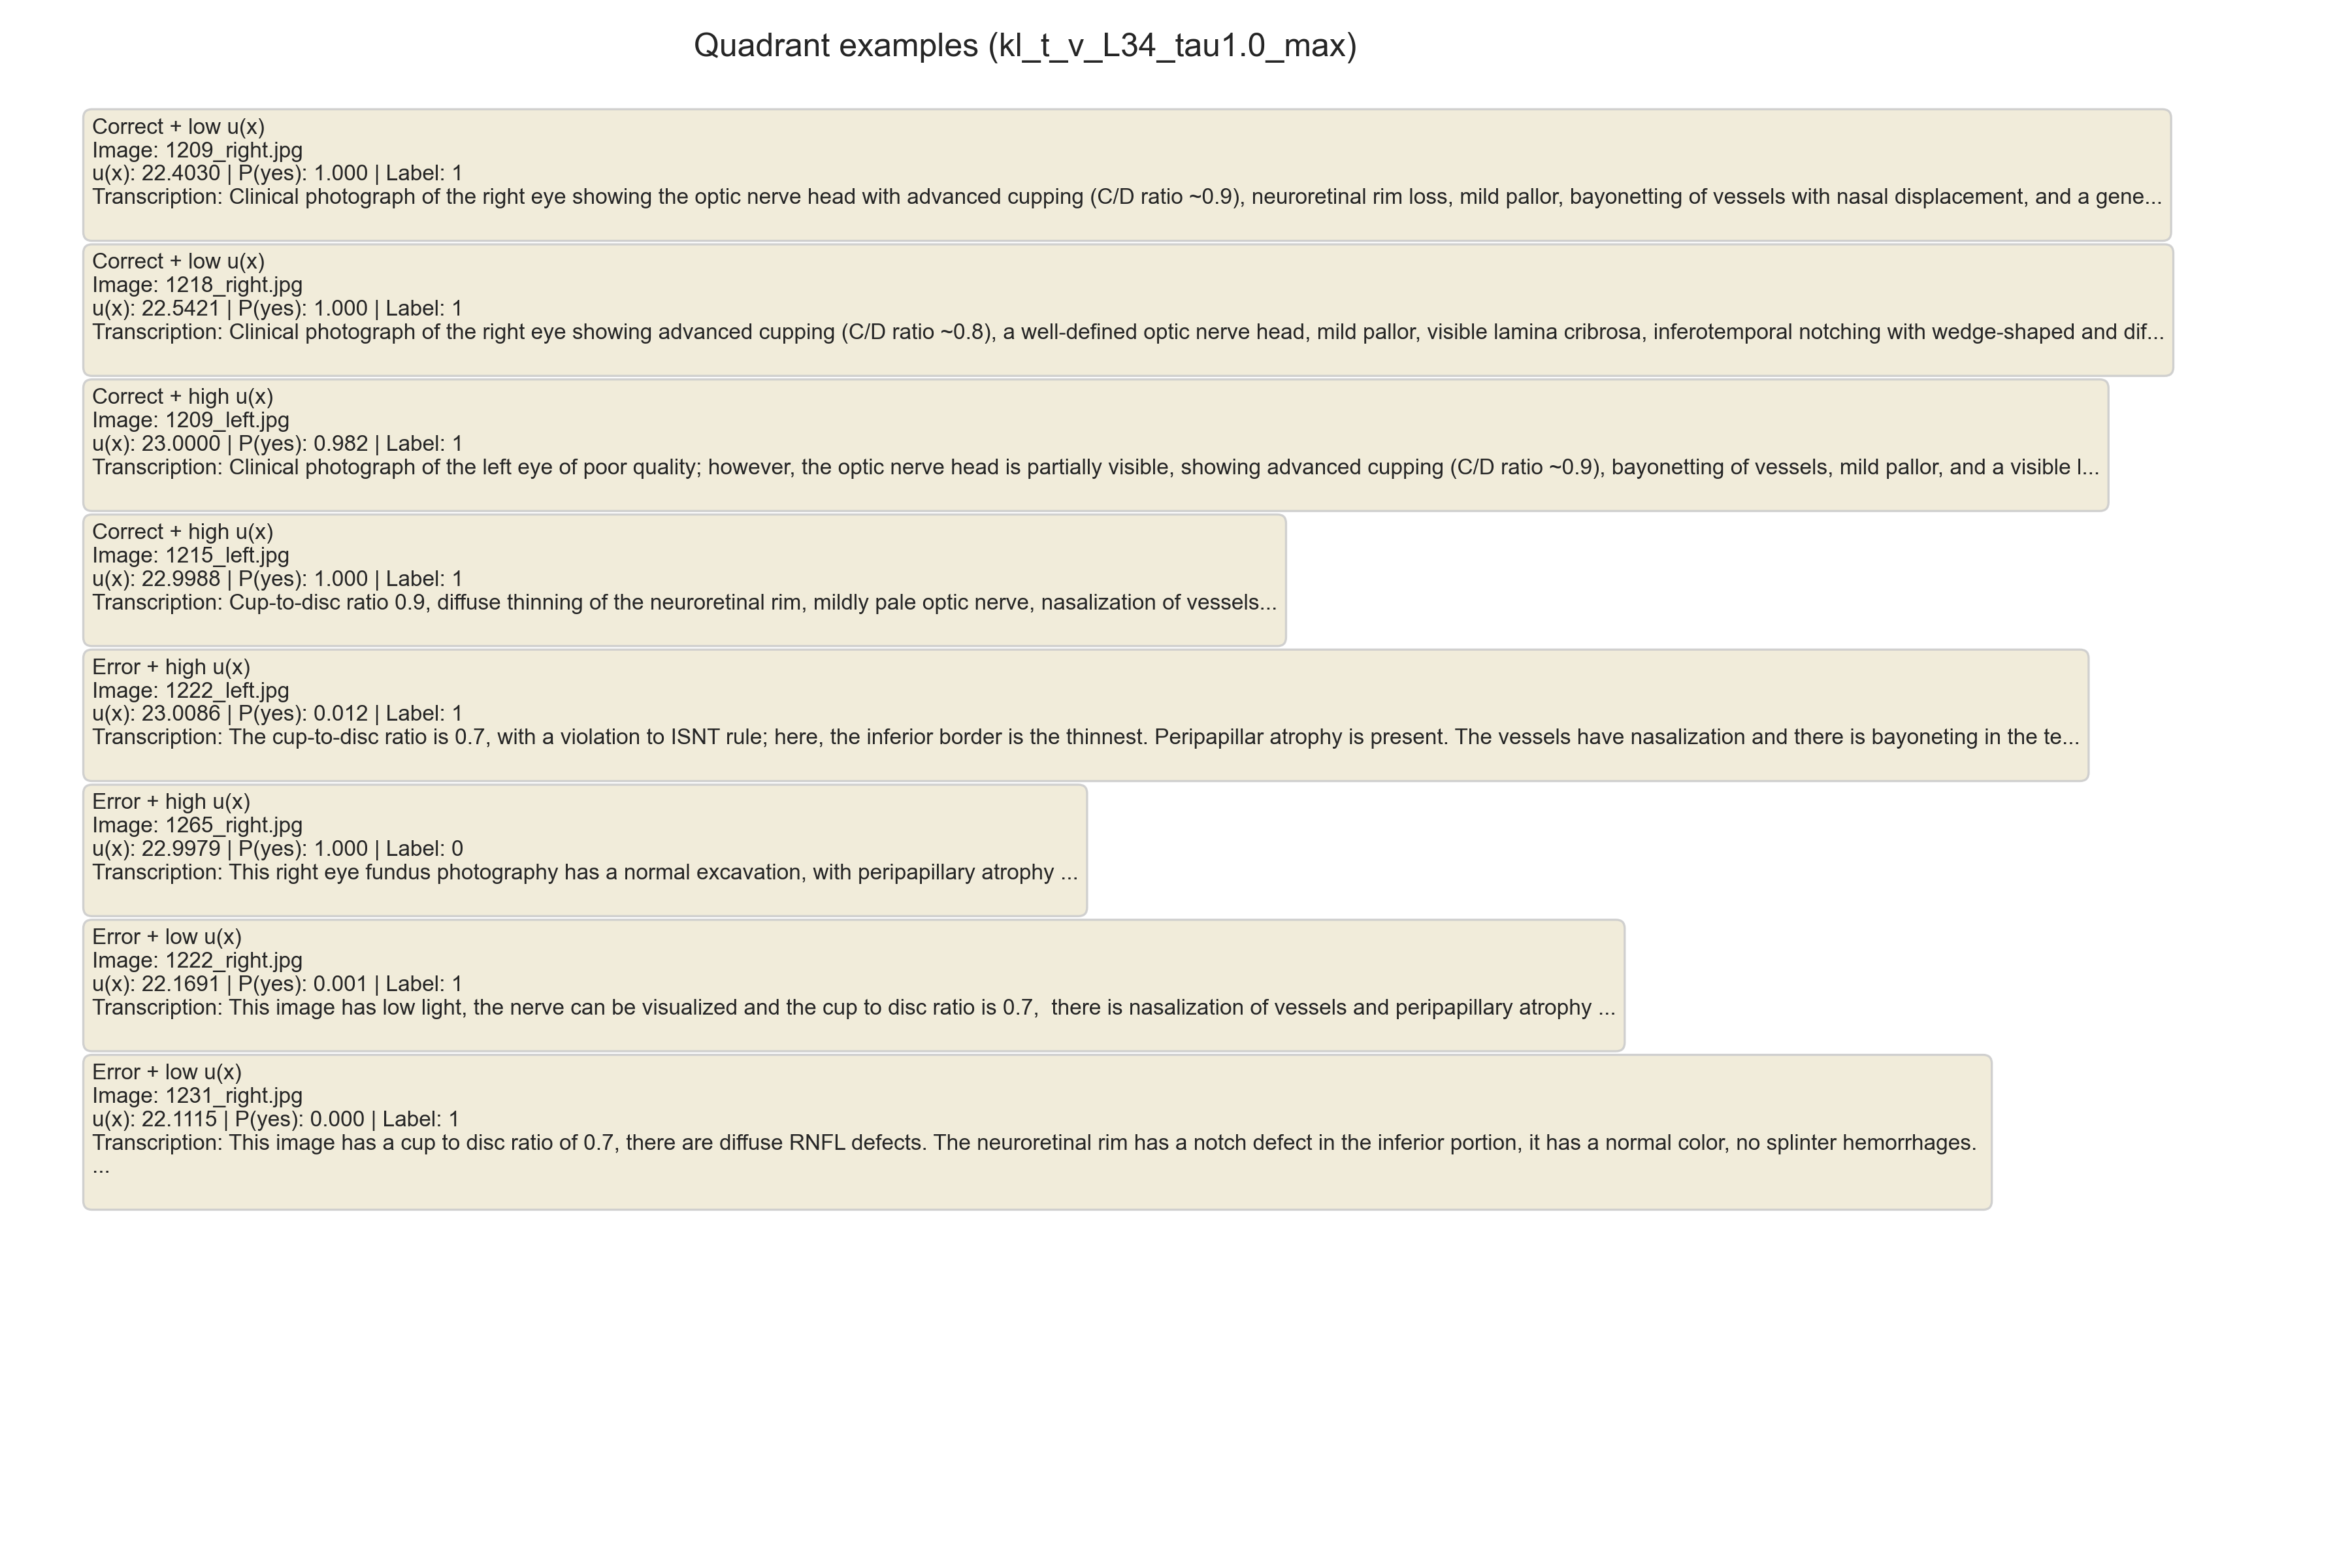
\includegraphics[width=\textwidth]{assets/fig5_quadrants.png}
    \caption{Los cuatro cuadrantes \texttt{correct} $\times$ $\ux$
    (alto/bajo) con ejemplos reales y la transcripción del oftalmólogo
    como referencia experta.}
    \label{fig:quadrants}
\end{figure}

Cruzar \texttt{correct} $\times$ $\ux$ con ejemplos reales muestra el
mecanismo en acción: \emph{correcto + baja u} (el caso típico, la cola
auto-respondible); \emph{correcto + alta u} (falsos positivos de la
alarma: copete fisiológico, miopía --- costo: derivaciones innecesarias);
\emph{error + alta u} (el cuadrante de oro: la alarma atrapa al modelo
equivocándose); \emph{error + baja u} (los errores más peligrosos:
sobreconfianza total; en esta cohorte son minoría --- de ahí la zona
verde --- pero existen y motivan la prudencia del esquema de 3 zonas).

\subsection{H4 (rechazada): la señal no mide severidad}
\label{sec:h4}

Correlación de Spearman entre $\ux$ y \texttt{cdr\_grade} en los 69
patológicos: $\rho = +0.001$, $p = 0.99$ (permutación). \textbf{H4
rechazada.} Interpretación importante: la KL responde a la dificultad
\emph{del modelo con el caso}, no a la gravedad clínica --- un glaucoma
avanzado y ``fácil de leer'' produce KL baja; un copete fisiológico benigno
pero ambiguo, KL alta. Para triage de errores del modelo es exactamente lo
que se quiere; para estratificación clínica de severidad, no sirve --- y
lo reportamos como resultado negativo con la misma prominencia.

% ============================================================
\section{Limitaciones y riesgos}
\label{sec:limitaciones}
% ============================================================

Reportamos las limitaciones con la misma prominencia que los resultados,
porque delimitan exactamente qué afirma y qué no afirma esta fase:

\begin{enumerate}[leftmargin=1.6em]
    \item \textbf{$N = 129$ es pequeño:} IC anchos ($\pm 0.10$--$0.13$);
    poder limitado para comparaciones pareadas.
    \item \textbf{AUROC $0.661$ es moderado:} no suficiente para
    deployment clínico directo; útil como componente de triage, no como
    decisor.
    \item \textbf{Un solo modelo y un solo dataset:} MedGemma-4B +
    MM-ODIR-129; la generalización a otros VLMs/tareas es conjetura
    (motiva la Fase 2).
    \item \textbf{H4 rechazada:} la señal no se correlaciona con severidad
    ($\rho = +0.001$, $p = 0.99$): detecta errores, no gravedad.
    \item \textbf{Confirmación val+test débil:} $0.569$ $[0.200, 0.938]$
    con solo 6 errores --- estadísticamente vacía.
    \item \textbf{Maldición del ganador:} Monte Carlo CV anidado $= 0.581
    \pm 0.116$ (KL sola) --- la generalización real está en
    $\sim$0.58--0.66.
    \item \textbf{SC evaluado en subconjunto de 50:} no comparable
    directamente con la cohorte; la comparación justa va etiquetada.
    \item \textbf{Verbalized degenerada:} solo 2 valores (90/95):
    posible limitación fundamental de VLMs instruction-tuned.
    \item \textbf{Heatmaps sin validación cuantitativa} contra las
    segmentaciones ground truth de copa/disco.
    \item \textbf{KL winsorizada:} techo $\ln(1/\varepsilon) = 23.03$
    nats; 24/129 imágenes por encima de 23.0 nats en la variante ganadora
    (el techo exacto solo se satura en la dirección espejo, 61/129) ---
    por diseño; los valores absolutos no son portables $\Rightarrow$
    derivación por percentil de cohorte.
    \item \textbf{Softmax restringido:} $p_{\mathrm{yes}}$ y MSP son
    scores binarios sobre 2 logits, no probabilidades calibradas de
    vocabulario completo.
    \item \textbf{Zona verde in-sample:} 30.2\% sin errores en ESTA
    cohorte; en pacientes nuevos el error esperado en la zona es
    $\lesssim 1/39$ (regla de tres, IC hasta $\sim$7.7\%).
    \item \textbf{Prevalencia curada} ($\sim$53\% patológicos vs.\
    $\sim$6\% en screening real): las métricas operativas no se trasladan
    directamente a población real.
    \item \textbf{Pendiente obligatorio antes de submission:} análisis de
    robustez excluyendo las imágenes con \texttt{has\_annotation\_artifact}
    (la flecha quemada de \texttt{1281\_right.jpg} es un potencial cue
    espurio; el análisis es un filtrado del CSV, sin re-cómputo).
\end{enumerate}

Riesgos técnicos registrados: \emph{massive activations} (regla float64
dura), dependencia de versión (\texttt{transformers} $\geq 4.51.3$),
sensibilidad al $\varepsilon$ del clamp (fijo entre corridas), y citación
anonimizada del dataset por doble ciego.

% ============================================================
\section{Conclusiones}
\label{sec:conclusiones}
% ============================================================

\begin{enumerate}[leftmargin=1.6em]
    \item \textbf{El desacuerdo cross-modal interno de un VLM médico es
    una señal real de alarma de error} (aunque moderada): AUROC $0.661$
    $[0.522, 0.772]$, $p = 0.006$, medida en una sola pasada y sin
    entrenar nada. H1 verificada; H2 parcial; H3 verificada en carácter
    exploratorio; H4 rechazada.
    \item \textbf{La fusión parameter-free por ranks con la confianza de
    salida es la mejor señal del estudio} (AUROC $0.698$; Excess-AURC
    $0.407$) y habilita un esquema de triage en tres zonas donde el 30.2\%
    menos incierto de la cohorte no contiene errores. Ambas combinaciones
    son contribuciones originales verificadas como sin precedente.
    \item \textbf{Los métodos que miran solo el output están ciegos en un
    modelo sobreconfiado:} la confianza verbalizada degenera (AUROC
    $0.519$, solo valores 90/95) y el self-consistency deriva fuera de
    formato ($0.655$, $p = 0.054$, costo 10$\times$). La información del
    error vive \emph{antes de la generación}, en los hidden states.
    \item \textbf{La generalización honesta} (Monte Carlo CV) ubica el
    desempeño en pacientes nuevos en $\sim$0.58--0.66 (KL sola) y
    0.648--0.698 (combinación): suficiente para proof-of-concept y para
    justificar la Fase 2; no para deployment clínico.
    \item \textbf{La verificación independiente es metodología doctoral
    permanente:} 19/19 checks con código independiente, logits bitwise
    reproducibles cross-GPU, y 8 bugs expuestos por controles
    estructurales que una lectura casual no habría atrapado.
\end{enumerate}

\paragraph{Próximos pasos inmediatos.} (i) Análisis de robustez excluyendo
artefactos de anotación (pendiente obligatorio); (ii) redacción del paper
IEEE BIP 2026 con citación anonimizada del dataset; (iii) Fase 2:
escalado a Harvard-FairVLMed y otros VLMs, siguiendo el roadmap de la
Sección~\ref{sec:roadmap}.

% ============================================================
% REFERENCIAS
% ============================================================
\begin{thebibliography}{99}
\small

\bibitem{abnar2020}
Abnar, S., \& Zuidema, W. (2020).
Quantifying attention flow in transformers.
\emph{Proceedings of ACL}.

\bibitem{azaria2023}
Azaria, A., \& Mitchell, T. (2023).
The internal state of an LLM knows when it's lying (SAPLMA).
\emph{Findings of EMNLP}.

\bibitem{beck2024}
Beck, M., et al. (2024).
UMPIRE: Uncertainty quantification for multimodal LLMs.
\emph{arXiv preprint}.

\bibitem{cormack2009}
Cormack, G. V., Clarke, C. L. A., \& Buettcher, S. (2009).
Reciprocal rank fusion outperforms Condorcet and individual rank learning methods.
\emph{Proceedings of SIGIR}.

\bibitem{farquhar2024}
Farquhar, S., Kossen, J., Kuhn, L., \& Gal, Y. (2024).
Detecting hallucinations in large language models using semantic entropy.
\emph{Nature}.

\bibitem{gal2016}
Gal, Y., \& Ghahramani, Z. (2016).
Dropout as a Bayesian approximation: Representing model uncertainty in deep learning.
\emph{Proceedings of ICML}.

\bibitem{geifman2017}
Geifman, Y., \& El-Yaniv, R. (2017).
Selective classification for deep neural networks.
\emph{Advances in NeurIPS}.

\bibitem{guo2017}
Guo, C., Pleiss, G., Sun, Y., \& Weinberger, K. Q. (2017).
On calibration of modern neural networks.
\emph{Proceedings of ICML}.

\bibitem{hullermeier2021}
Hüllermeier, E., \& Waegeman, W. (2021).
Aleatoric and epistemic uncertainty with random forests.
\emph{Machine Learning}.

\bibitem{kuhn2023}
Kuhn, L., Gal, Y., \& Farquhar, S. (2023).
Semantic uncertainty: Linguistic invariances for uncertainty estimation in natural language generation.
\emph{Proceedings of ICLR}.

\bibitem{lakshminarayanan2017}
Lakshminarayanan, B., Pritzel, A., \& Blundell, C. (2017).
Simple and scalable predictive uncertainty estimation using deep ensembles.
\emph{Advances in NeurIPS}.

\bibitem{leng2024}
Leng, S., et al. (2024).
Mitigating object hallucinations in large vision-language models through visual contrastive decoding (VCD).
\emph{Proceedings of CVPR}.

\bibitem{li2023}
Li, C., et al. (2023).
LLaVA-Med: Training a large language-and-vision assistant for biomedicine in one day.
\emph{Advances in NeurIPS}.

\bibitem{luo2024}
Luo, Y., et al. (2024).
FairCLIP: Harnessing fairness in vision-language learning (Harvard-FairVLMed).
\emph{Proceedings of CVPR}.

\bibitem{sellergren2025}
Sellergren, A., et al. (2025).
MedGemma technical report.
\emph{Google Research}.

\bibitem{vovk2005}
Vovk, V., Gammerman, A., \& Shafer, G. (2005).
\emph{Algorithmic learning in a random world} (Conformal Prediction).
Springer.

\bibitem{wang2022}
Wang, X., et al. (2022).
Self-consistency improves chain of thought reasoning in language models.
\emph{Proceedings of ICLR}.

\end{thebibliography}

\end{document}
